% Break apart the applications graph for epidermal robots
% Add the mechanical testing 
% Summary/breakdown of application space
% Add 3D printing on the body
% Add suction cups testing with IR sensor inside. 
\chapter{Applications}
This chapter provides potential applications of DWT in three areas: physiological sensing, human-computer interactions, and design. The applications for Epidermal robots were designed to highlight their access to the skin and physiological sensing. The applications of Rovables highlights human-computer interactions. 
% Medical
% HCI 
% Application scenarios
% Non-wearable applications - wall inspection
% Ideal scenario?
% Table of applications? 
%\section{Scenarios}
\section{Physiological sensing}
DWT robots can sense noninvasively physiological data on human skin. Some of them, such as skin mechanical properties and biopotentials, can be sensed directly by the suction cups. This is especially useful in medical sensing. Currently, most of such tests are performed manually by a doctor; therefore, they are hard to perform consistently. Furthermore, the doctor is limited by the human senses of touch, vision, and sound. The robot can test things outside of that range. 

\subsection{Skin mechanical properties}
The epidermal robots can directly test the mechanical property of skin directly underneath them. This is done by applying a mechanical stimulus on the skin and measuring a response. We created two prototypes that push on the skin and pull on the skin. 

Currently, such tactile sensing can be done using a robot arm with a sensor tip~\cite{kawasaki2002dexterous}, as a hand-held~\cite{wellman2001tactile} or stationary instrument or by hand.  Providing exact measurements with those methods is challenging as such sensing requires applying force on the skin. The body is not rigid and has many flexible joints, therefore need to be fixed entirely. For example, if a robot arm pushes on the skin, it will create an equal reaction force. The epidermal robots are attached locally, so all the effects are created in a small area. The body parts do not need to be rigidly fixed. 



\begin{figure}[!t]
\centering
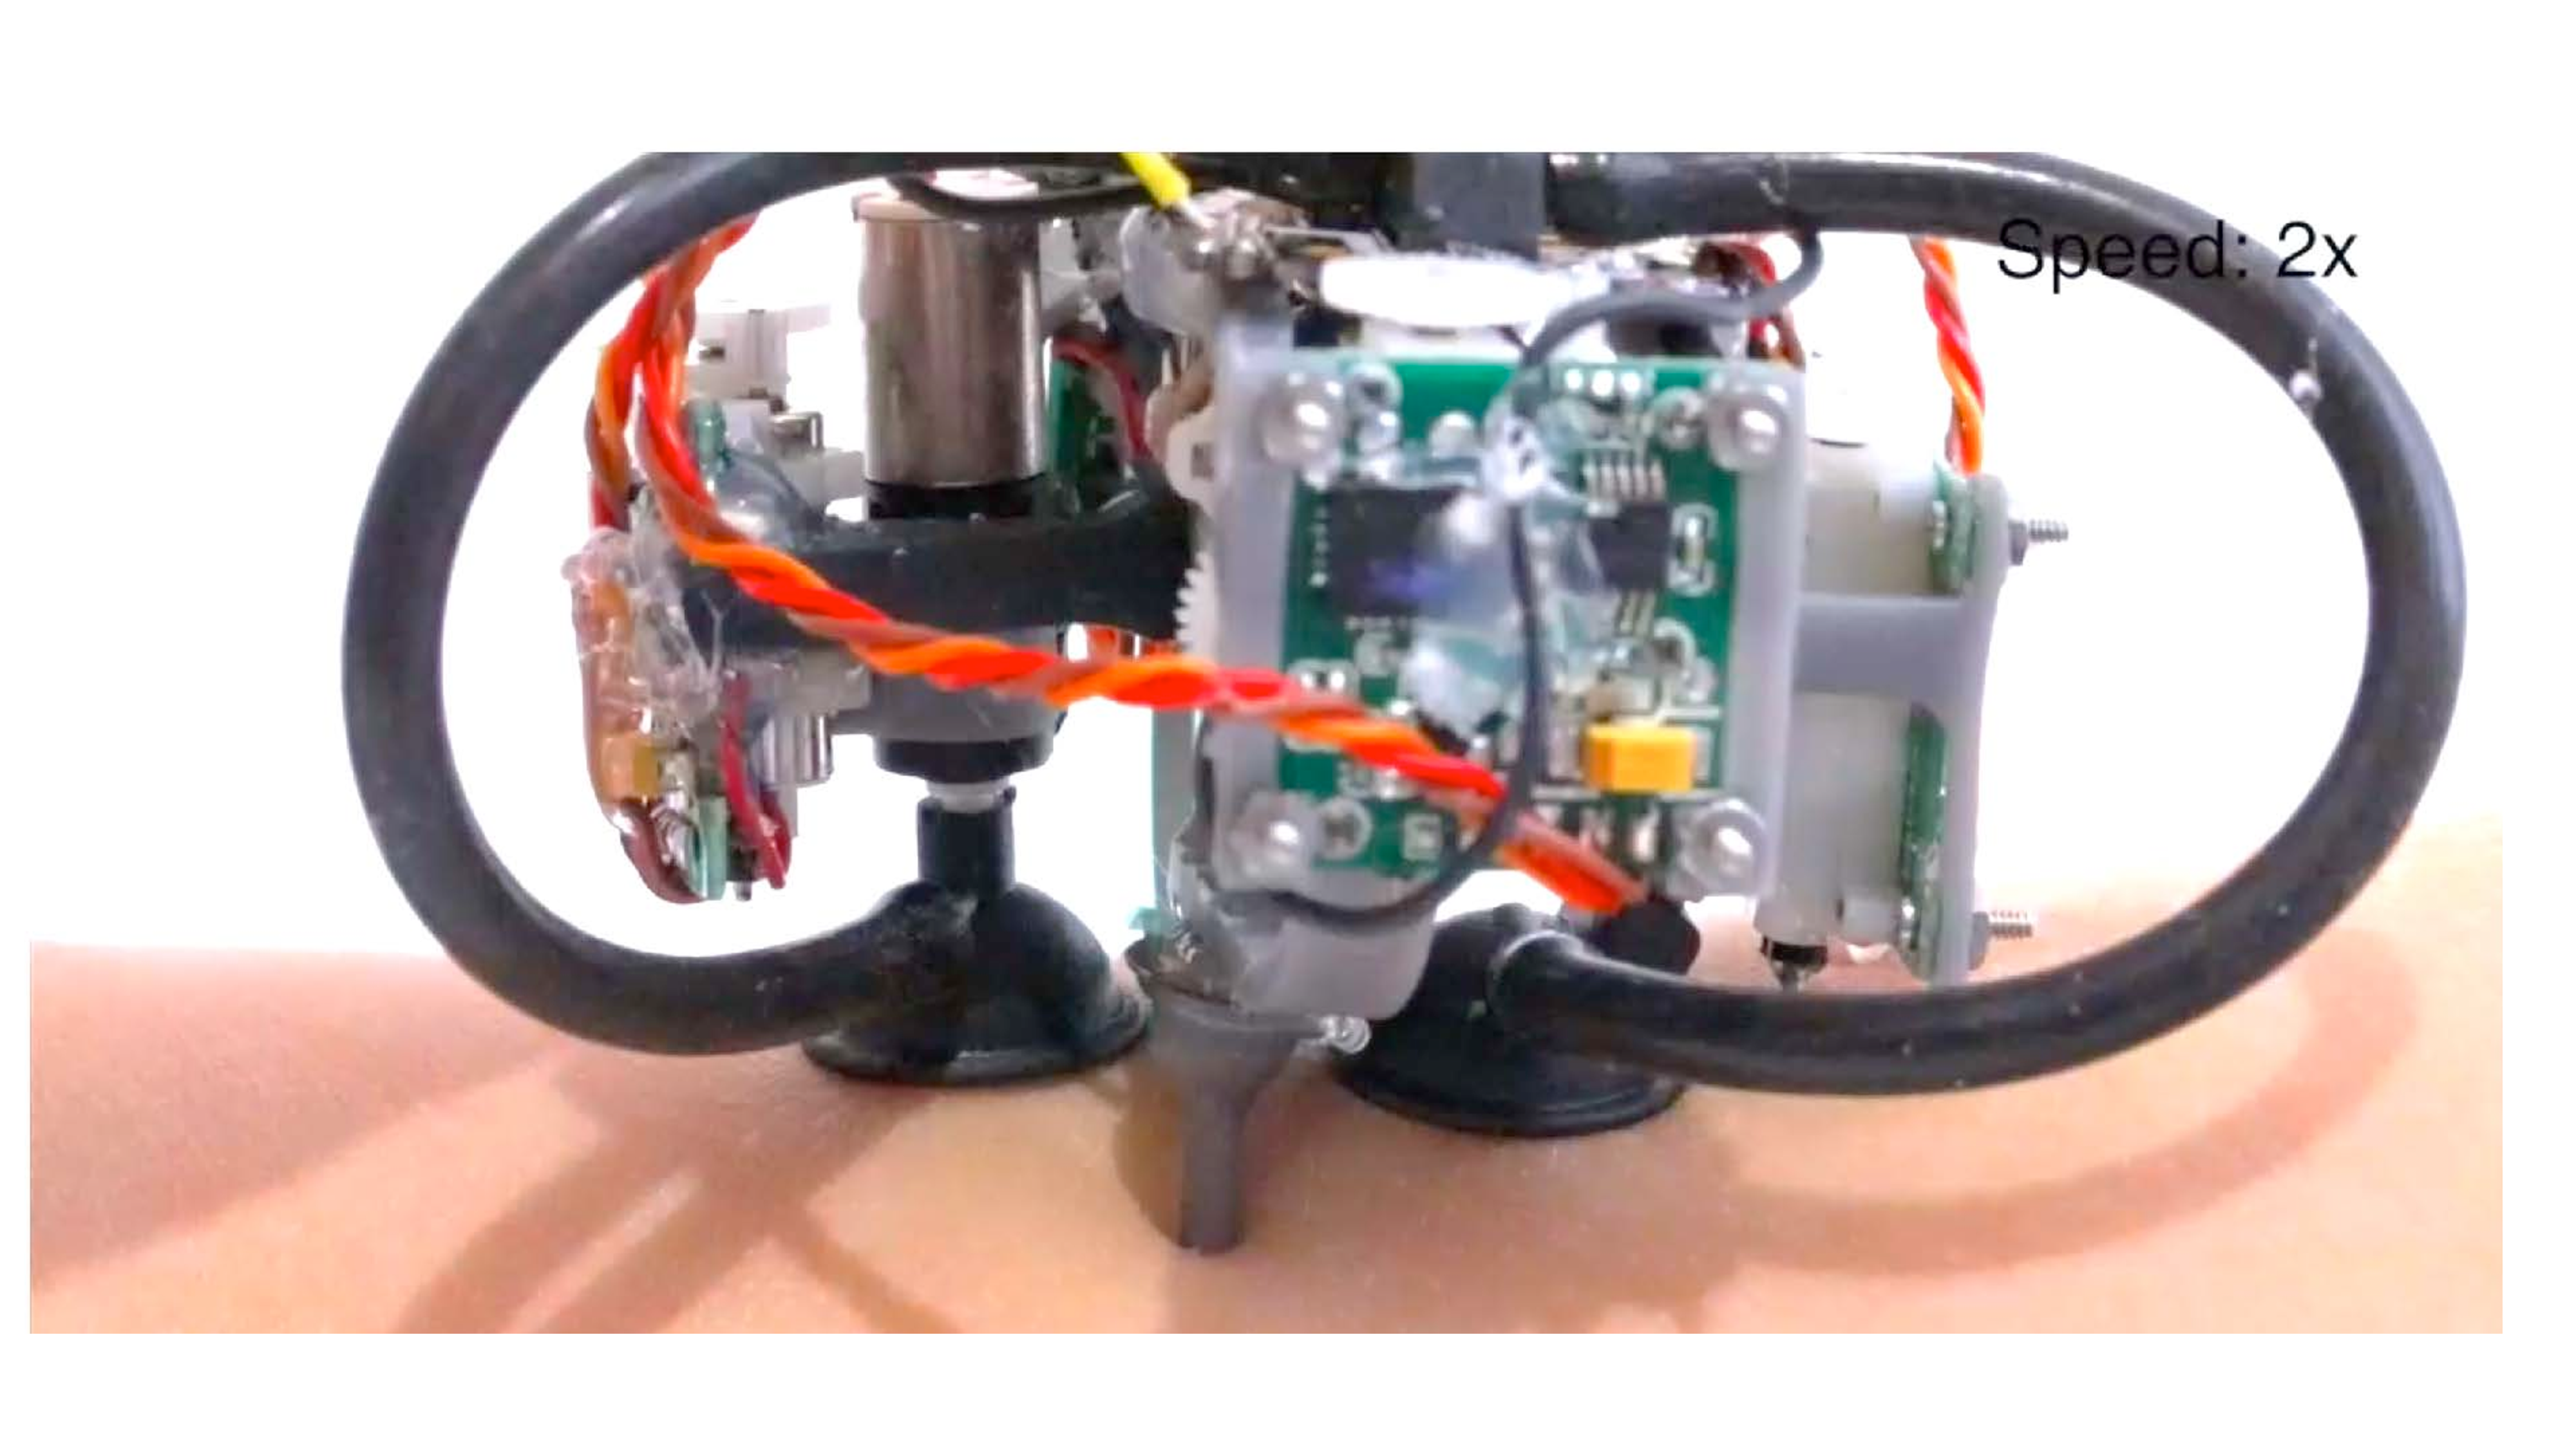
\includegraphics[width=10.0cm]{pictures/applications/pushing_robot.pdf}
\caption{The epidermal robot equiped with a plunger to test mechanical properties of the skin. In this picture, the robot is attached to forearm.}
\label{fig:pushing_robot}
\end{figure}


\subsubsection{Stiffness testing instrument design}
Pushing on the skin provides information about the hardness of the skin, and can be used to derive Young's modulus\footnote{Stiffness defined by stress/strain ratio in the material's linear region}.  This is similar to an instrument called durometer, which creates an indentation in the material to identify their hardness quickly. We equipped the robot with two vertical linear servo motor (SPMSA2005, Spektrum) and a rod that pushed on the skin, as shown in Figure~\ref{fig:pushing_robot}. We used two motors to increase the pushing force as well to position the rod between the two suction cups. If the rod were offset from the middle, the robot would tilt during the pushing, and potentially causing detachment from the skin. 
The displacement of the rod was extracted by digitalizing the voltage from the potentiometer of the servo, used for position feedback. This provided the strain measurement. The strain was unitless, as it was divided by initial strain. To measure the stress (Newton), we added an FSR (force sensitive resistor) to the tip of the rod. An identical 0.2inch FSR sensor (FSR400, Interlink), was used in my previous work to sense gestures from wrist motions~\cite{dementyev2014wristflex}. We calibrated the FSR with a digital scale (SCM2600, My Weight) to convert arbitrary voltage divider readings from FSR into Newtons.
Figure~\ref{fig:youngs_modulus} shows the data obtained from the robot pushing on the skin. The slope of the stress vs. strain graph is defined as Young's Modulus. 

The robot has to be reasonably well and stably attached to the skin, as the force exerted by the rod into the skin is transferred to the suction cups. To prevent detachment this force has to be less than the attachment force of the robot.

\subsubsection{Custom wearables}
Mapping the hardness of the human body has useful applications. For example, it can be used to manufacture more comfortable and efficient prosthetics using multi-material 3D printers. Ideally the prosthetic should have variable stiffness to match the elasticity of the limb, but this requires a prior map of elasticity~\cite{lin2017low,moerman2009digital}. The current measurement tools require a large mechanical apparatus or multiple camera setup.  The DWT robots can be used to map the stiffness at home without the need for large machines. 

\begin{figure}[!t]
\centering
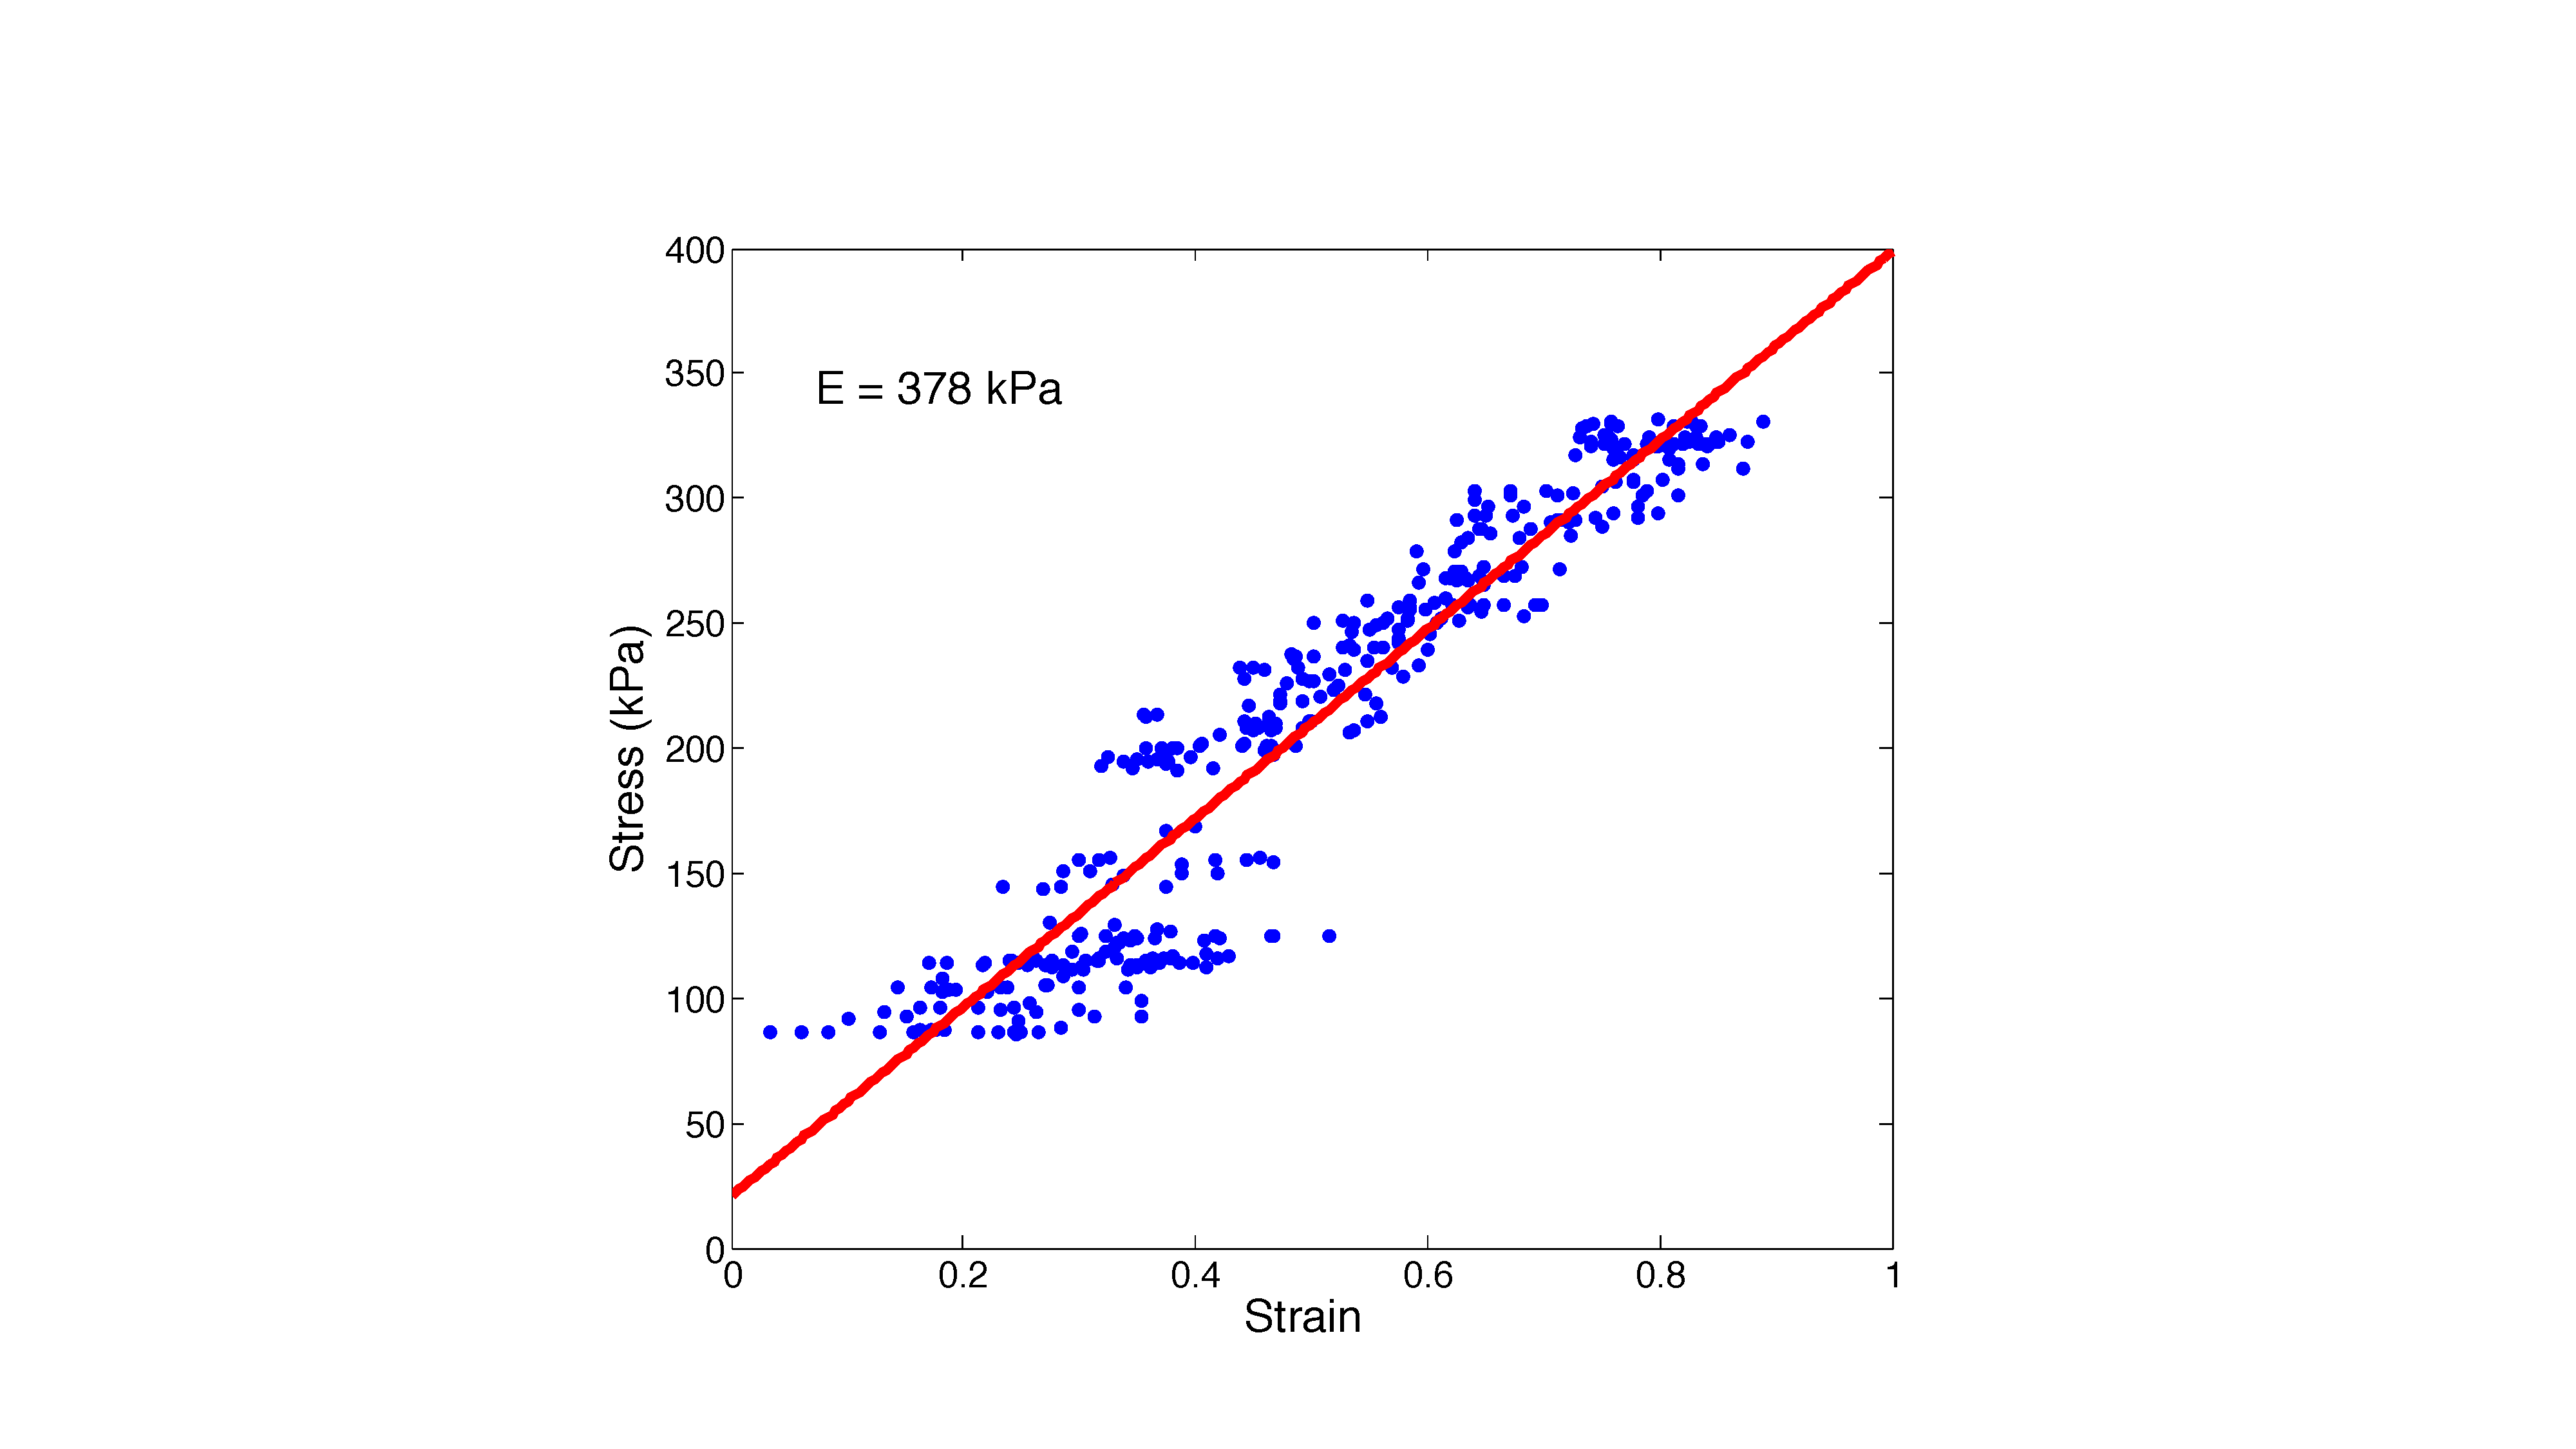
\includegraphics[width=10.0cm]{pictures/applications/young_modulus_graph.pdf}
\caption{Stress vs. strain graph obtained from pushing the skin on the arm. The red line is the slope, which was used to obtain Young's modulus.}
\label{fig:youngs_modulus}
\end{figure}

Knowing the stiffness can also allow for more comfortable wearable devices. As shown in Figure~\ref{fig:arm_brace}, we made a concept of a 3D printed (Form 2 with durable resin, Formlabs) arm brace that used 3D map and stiffness data. The stiffness was varied by changing the size of the cells in the mesh.

\begin{figure}[!t]
\centering
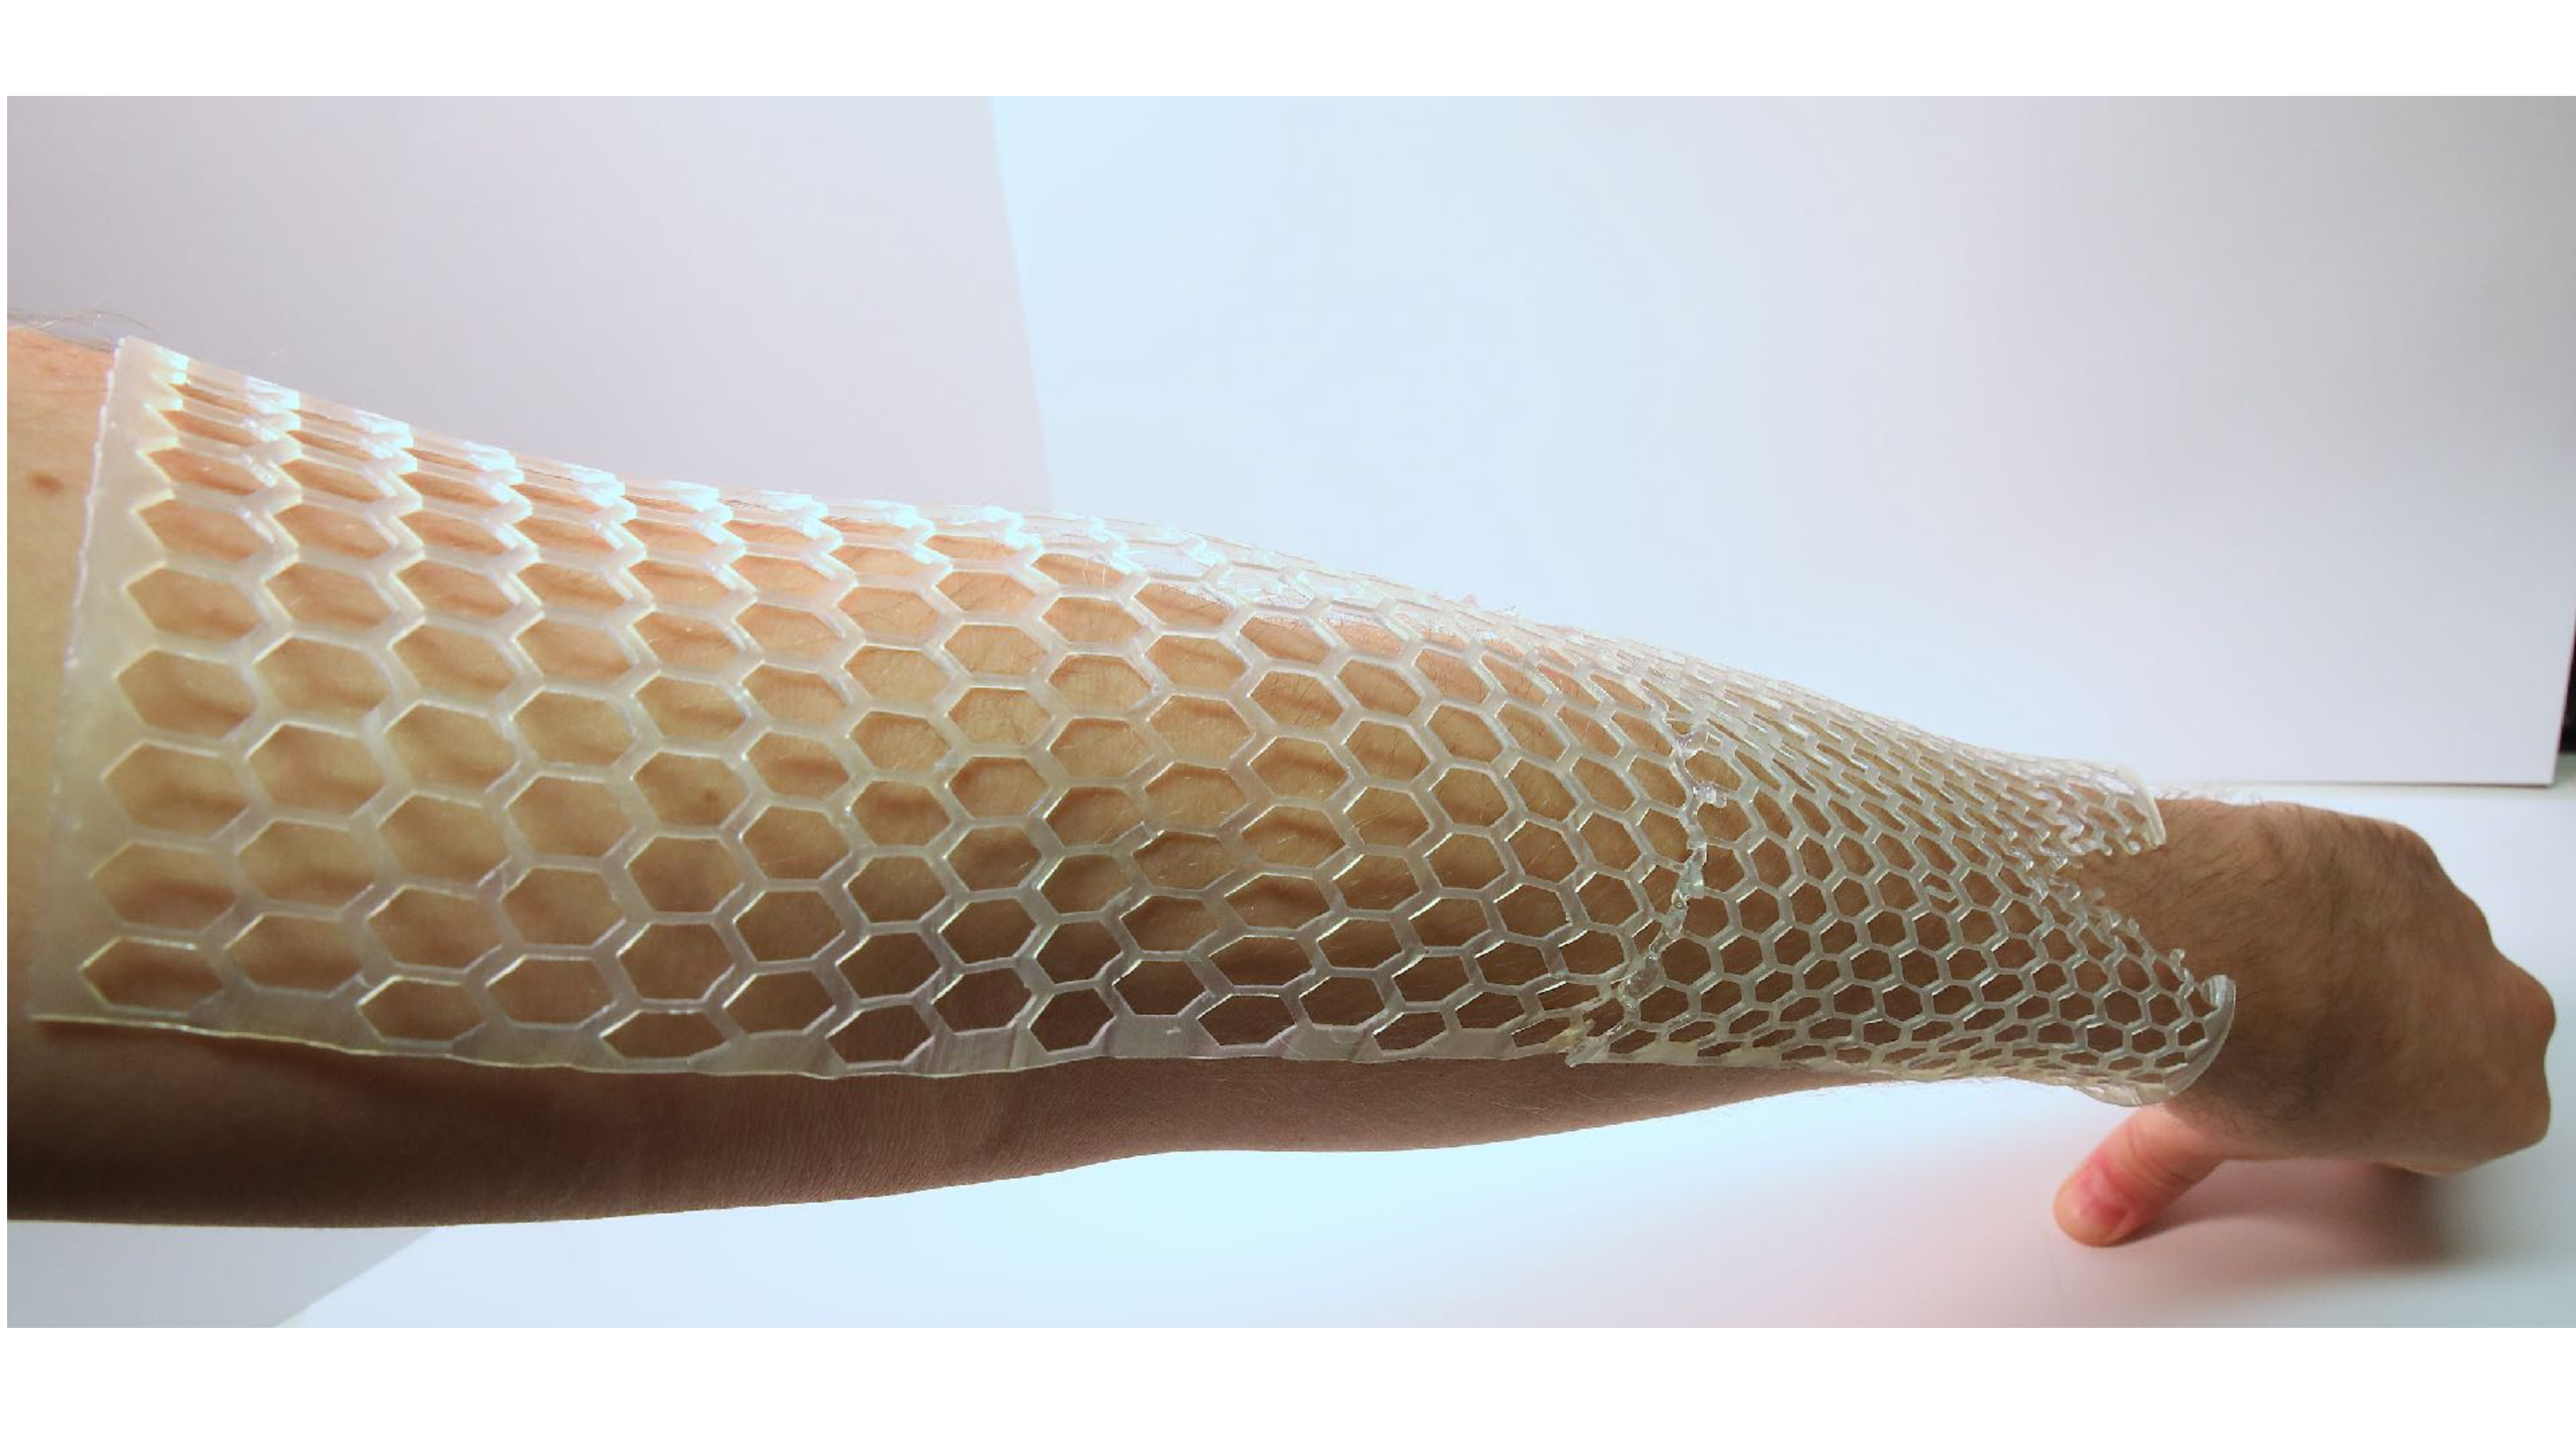
\includegraphics[width=1\columnwidth]{pictures/applications/arm_brace.pdf}
\caption{3D printed arm brace with different stiffness segments.}~\label{fig:arm_brace}
\end{figure}

\subsubsection{Disease testing and prognosis.}
% Add Mechanical Imaging of Soft Tissues with a Highly Compliant Tactile Sensing Array
Also, measuring the stiffness is useful in early disease detection. Many disorders change the mechanical properties of the skin or underlying tissues. For example, lymphoma~\footnote{cancer of lymph nodes} presents itself as lumps under the skin. The detection is done by the doctor by feeling the tissue with hands~\cite{de2002early}. Such a measurement method is not systematic and largely depends on the doctor. Furthermore, research has shown that robotic tactile sensor can be more sensitive than human touch in skin lumps detection~\cite{gwilliam2010human}. A tactile handheld sensor is useful in measuring the mass size of a breast lumps.~\cite{wellman2001tactile}

Pulling on the skin also provides information about tissue's mechanical properties. This technique is often used in cosmetics and skin care industry to understand the effect of different skin products. A tool called Cutometer is used to pull on the skin using vacuum and simultaneously measures how far the skin is pulled~\cite{dobrev2000use}. With Epidermal Robots this technique is straightforward to implement, as robot already uses suction for attachment. We added a infrared proximity sensor (GP2S60A, Sharp) inside the suction cup to measure the skin's bulging. An example of data of skin deformation in the suction cup is shown in Figure~\ref{}. 
% Pic of robot with IR measuremnt
% Pic of IR measurement map

Multiple measurement techniques can be used simultaneously to provide better results. The robot can combine both pushing and pulling on the skin, as well as optical imaging to collect more information. 

\begin{figure}[!t]
\centering
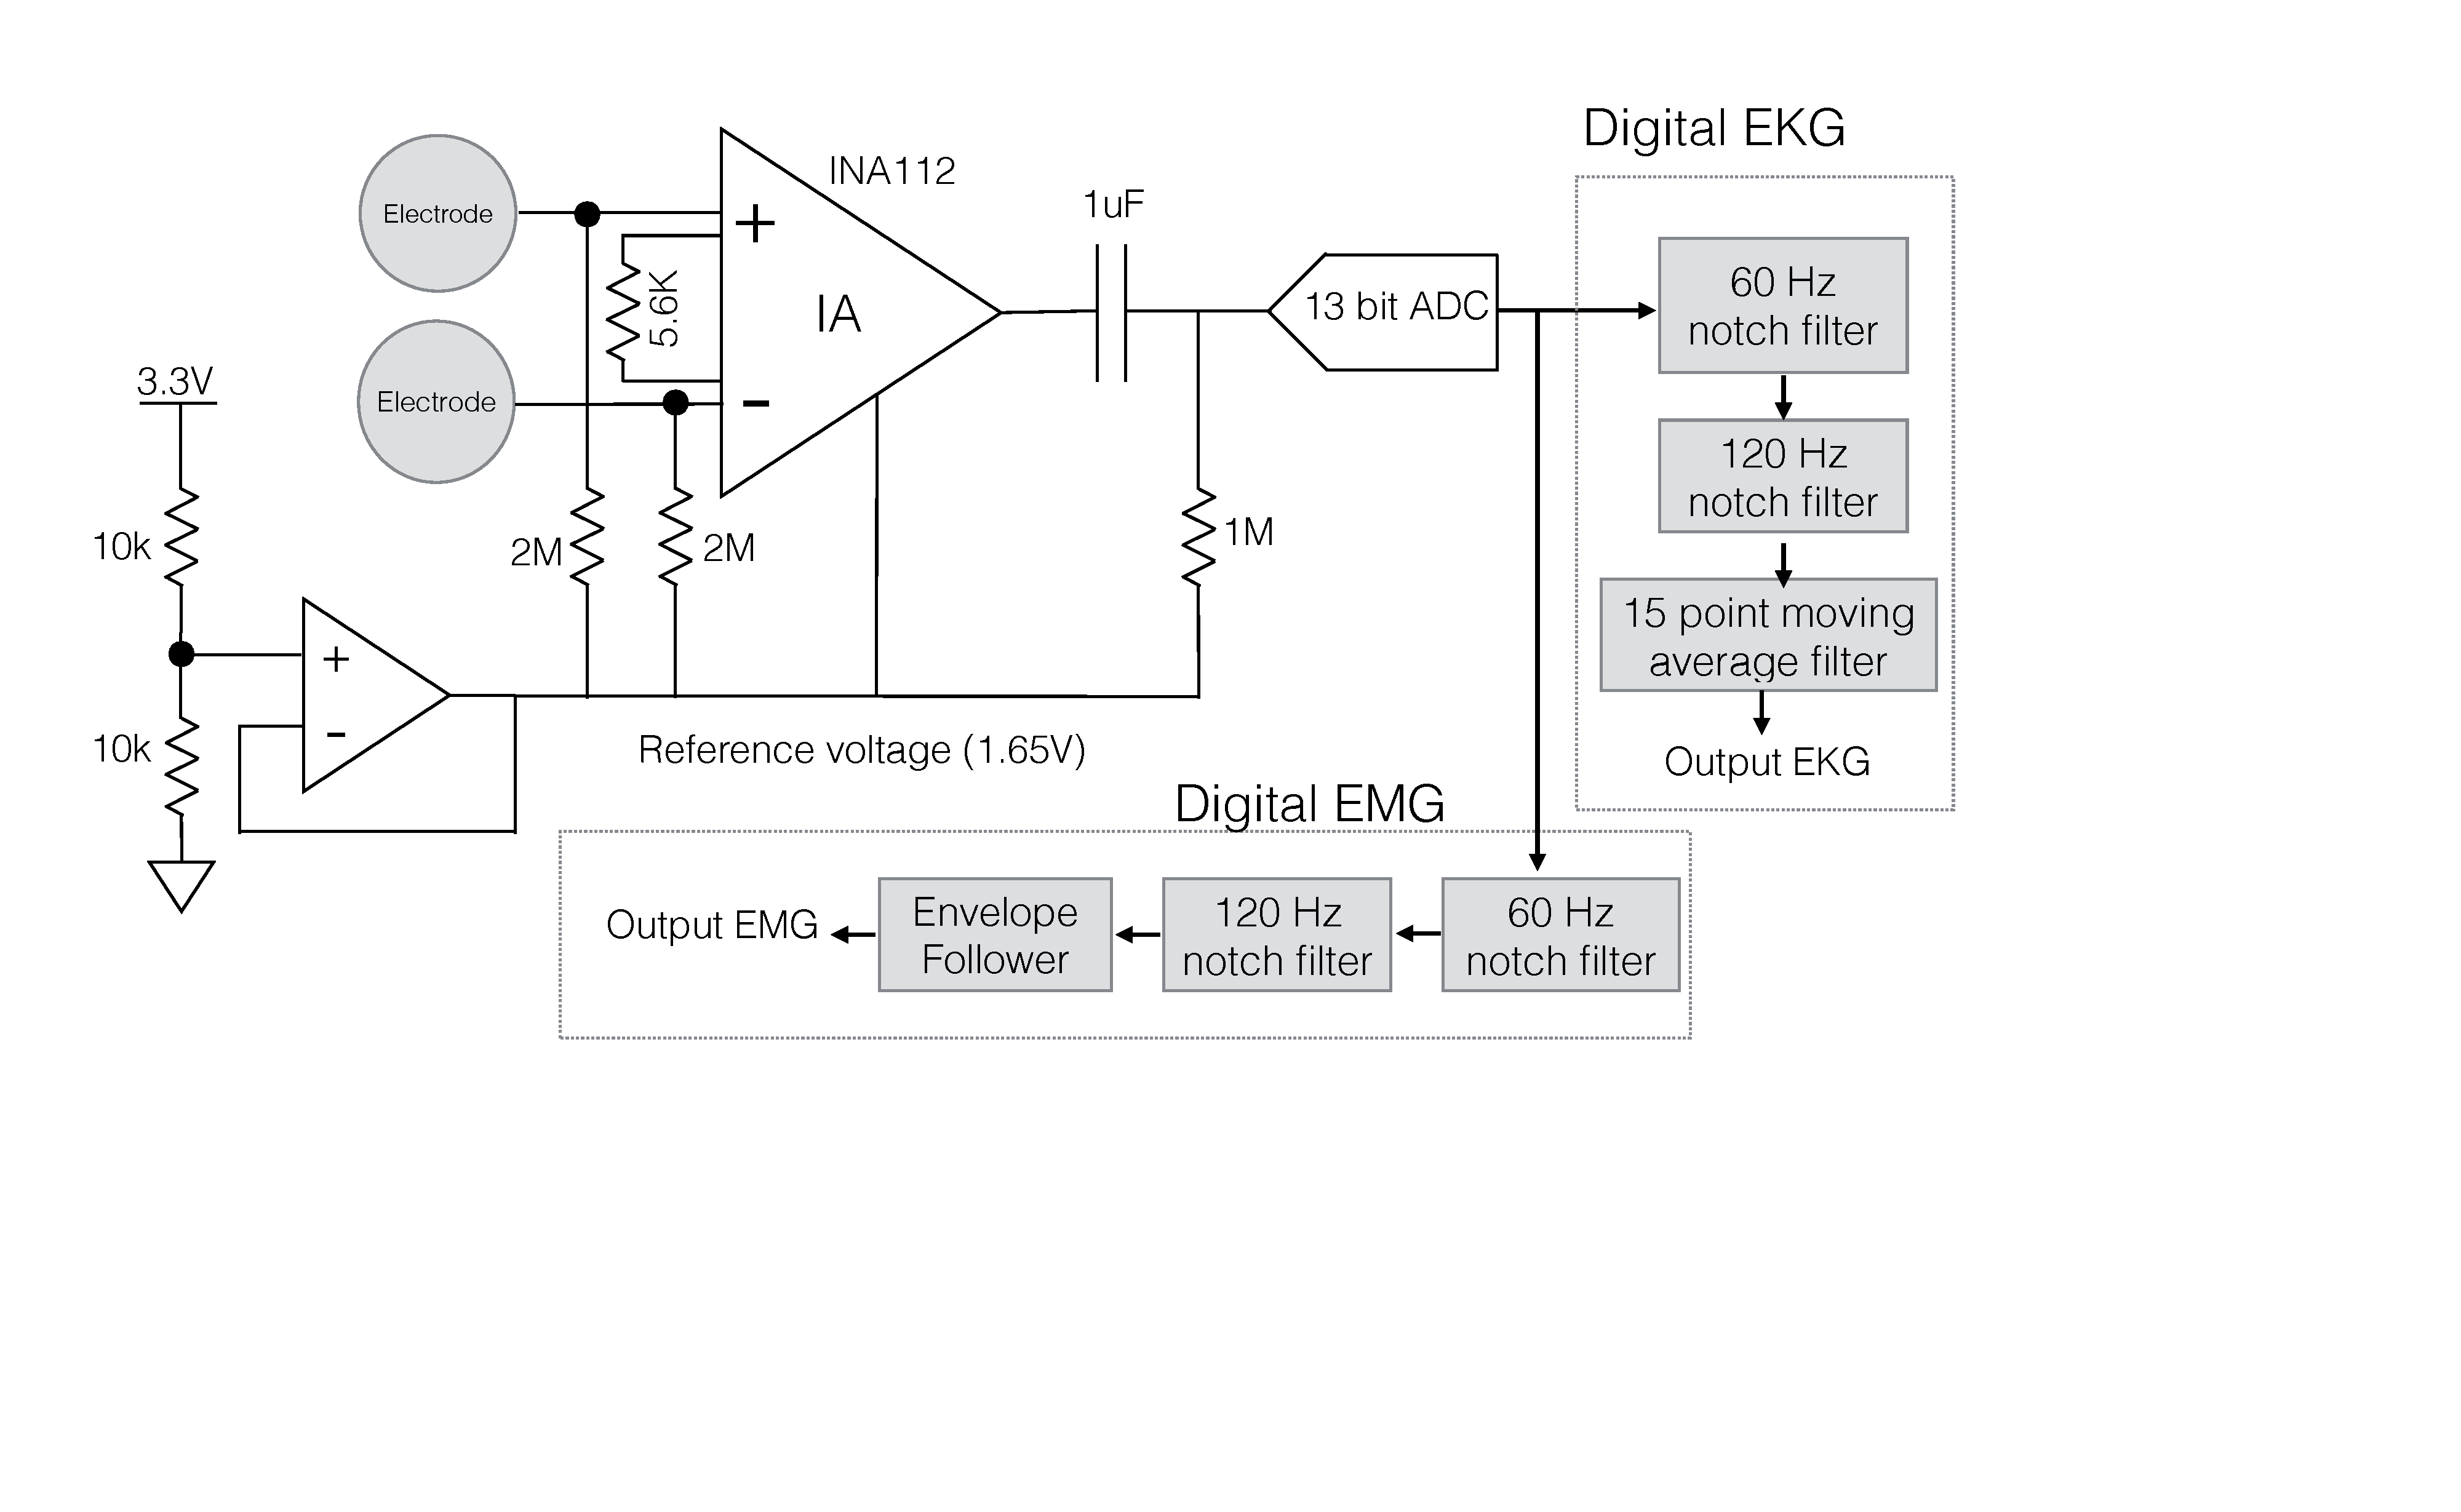
\includegraphics[width=10.0cm]{pictures/chapter3/biopotential_circuit.pdf}
\caption{The biopotentials pickup circuit diagram. EMG and EKG had the same analog front end: instrumentation amplifier with a gain of 10. The amplifier followed by a high pass filter of 0.16 Hz, which removed the DC baseline. To capture the complete signal shapes, the circuit was referenced to 1.65V (half of the supply). }
\label{fig:biopotential_circuit}
\end{figure}

 %Biopotential sensing
\begin{figure}[!t]
\centering
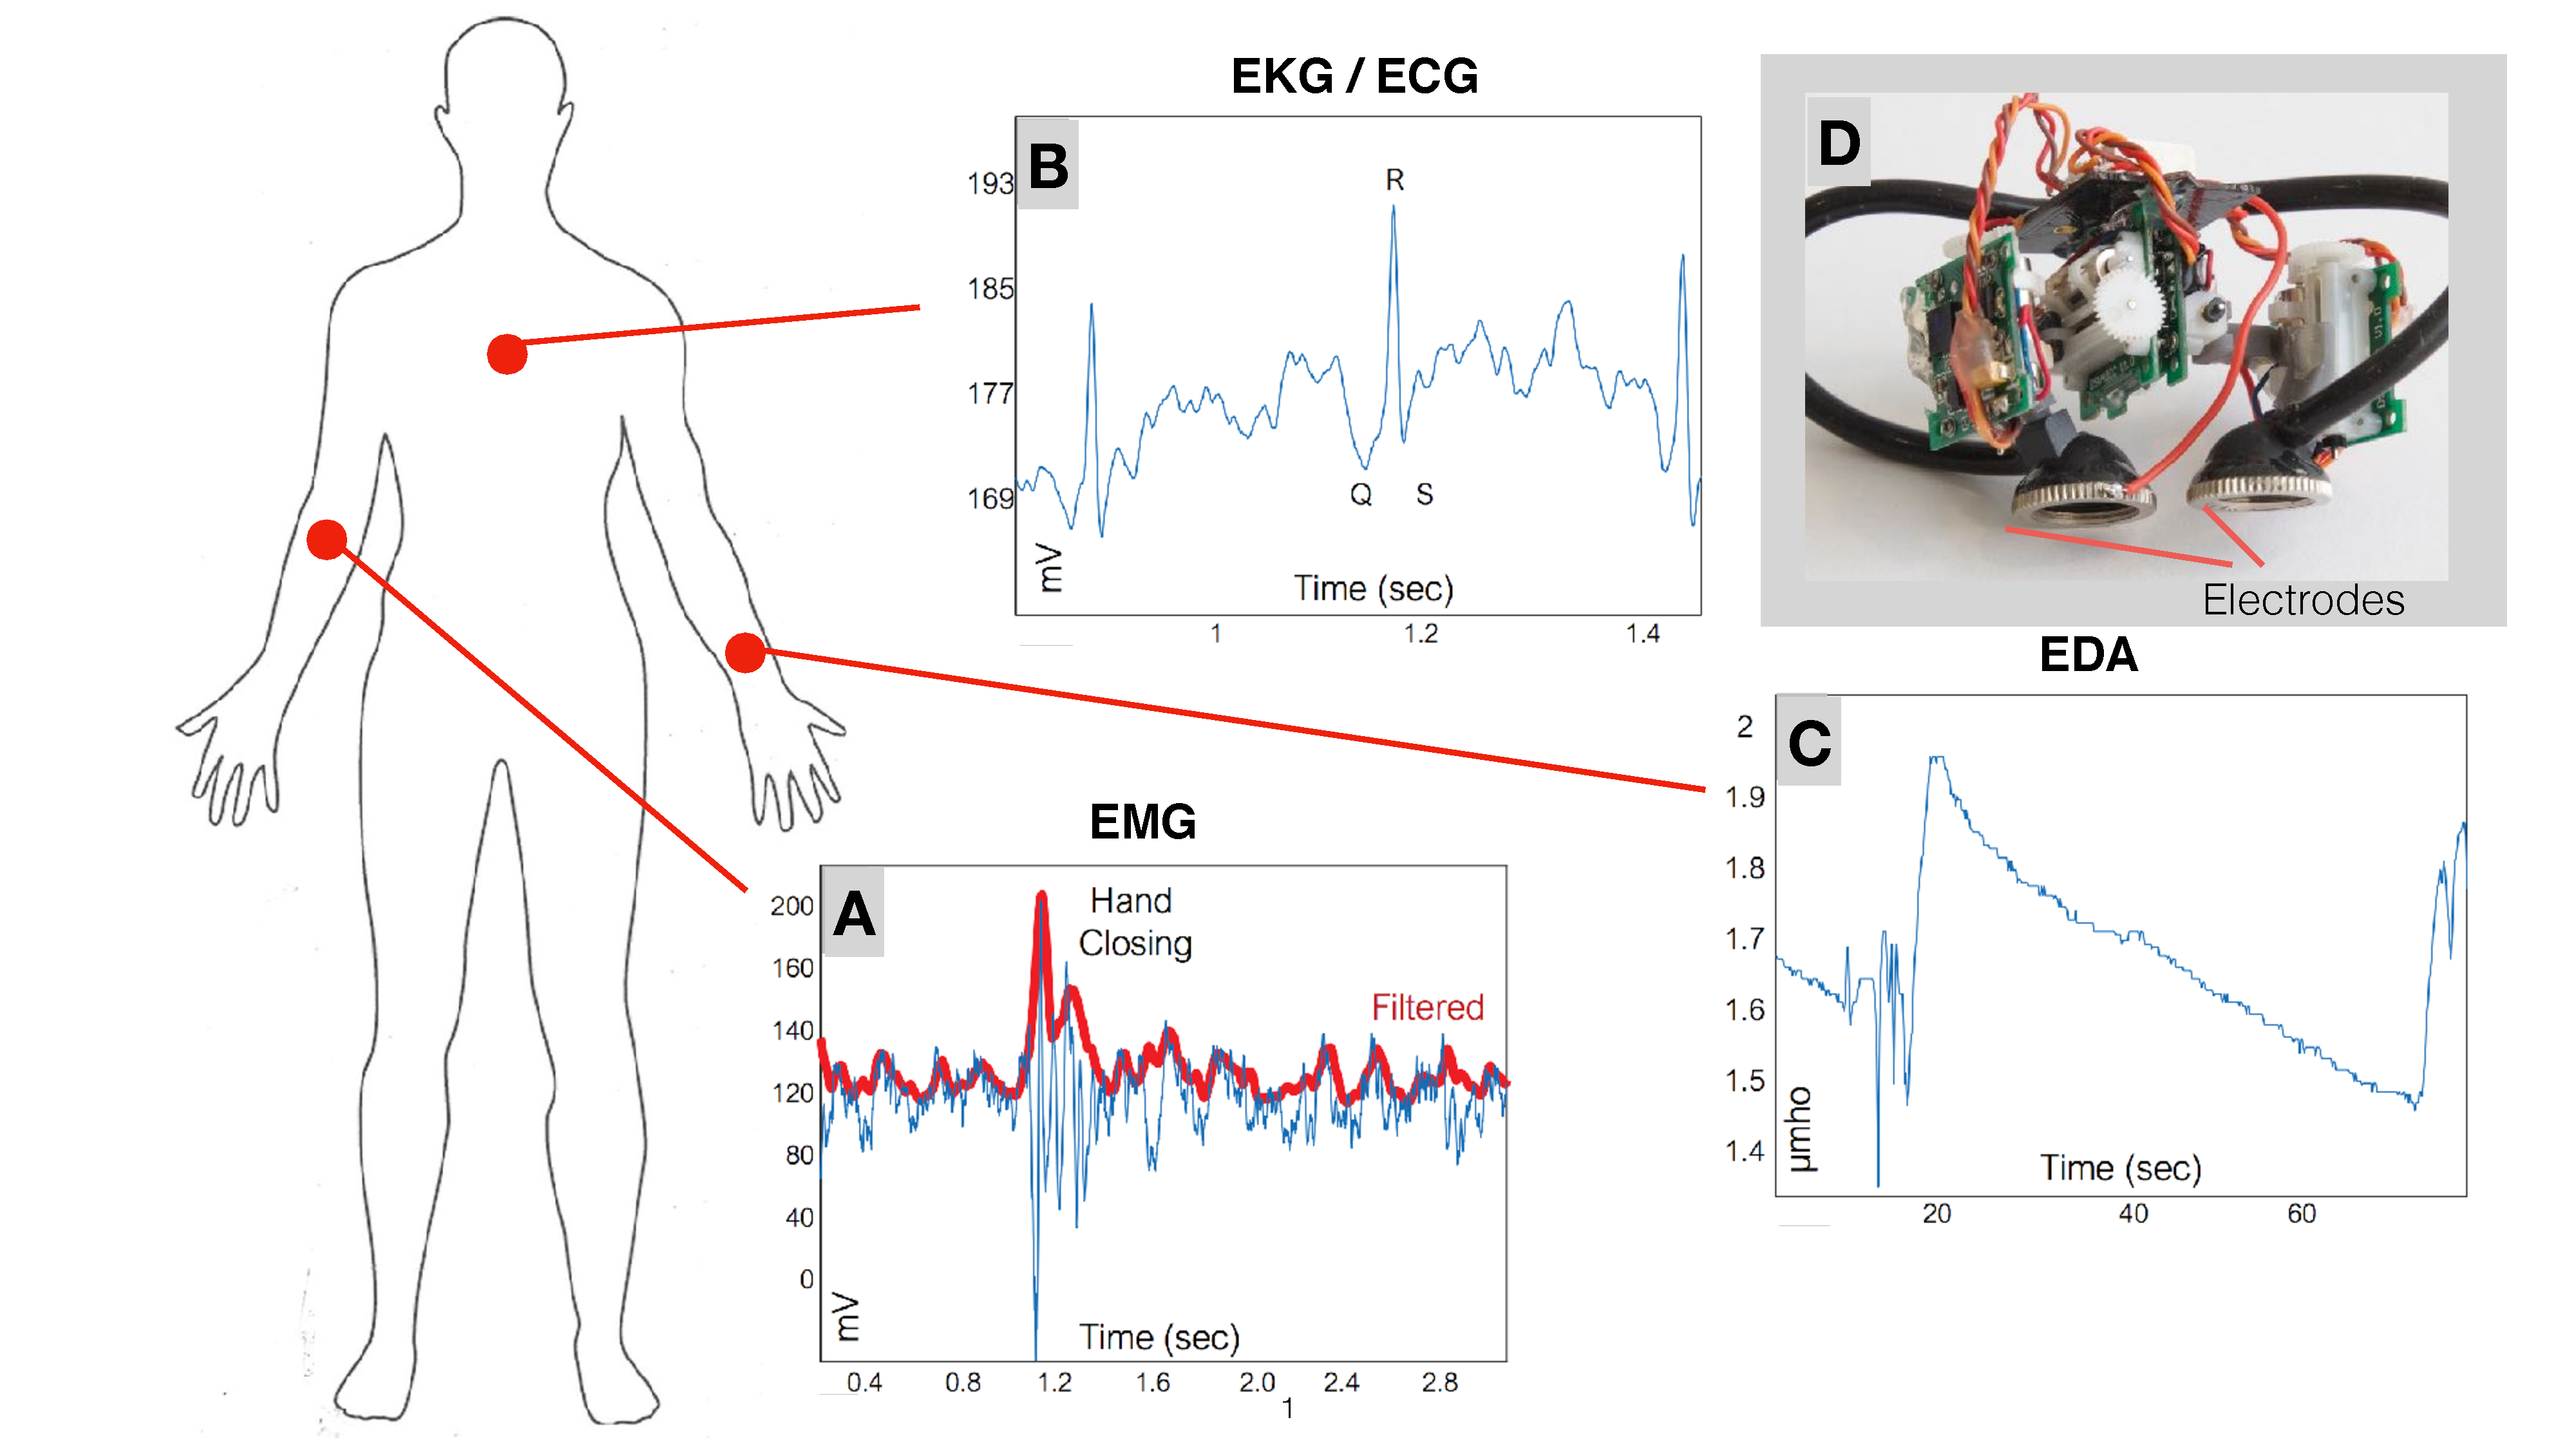
\includegraphics[width=1\columnwidth]{pictures/applications/biopotential_sensing.pdf}
\caption{Biopotential sensing: A), Electromyographic signal measured on the upper arm when closing the hand. B), Electrocardiographic (EKG) signal measured on the chest showing the QRS complex, C), Electrodermal activity signals on the wrist in
response to an auditory stimulus. D), Side view of SkinBot showing the modified suction-cups to monitor the electrical properties of the skin. 
Visual Imaging (middle row):}~\label{fig:biopotential_sensing}
\end{figure}

\subsection{Biopotentials}
SkinBot contains an implementation of a circuit to monitor the electrical properties of the skin. To do so, we glued stainless steel washers (ID=9.0mm, OD=12mm, thickness=2mm) around the suction cups so they could also serve as electrodes. The electrodes can be used to capture electrocardiograms from the chest (ECG), electromyographic signals of the muscles (EMG), and electrodermal activity (EDA) from areas of the body where the density of eccrine sweat glands is dense (e.g., wrists, upper arm)~\cite{boucsein2012electrodermal}. As the robot moved to different locations, Figure~\ref{fig:biopotential_sensing} shows EMG, ECG, and EDA traces captured from the chest, upper arm, and the interior part of the wrist, respectively. The detailed biopotential circuit diagram is shown in Fig.~\ref{fig:biopotential_circuit}. 

To capture biopotentials, we used an instrumentation amplifier (INA114, Analog Devices) as front-end to reject the residual 60Hz noise. A 0.16Hz high-pass filter provided DC drift rejection, and 30Hz low-pass filter provided a further 60 Hz noise rejection. We used quad op-amps (MCP6044, Microchip) for voltage reference and filtering. The data were digitized at 976 Hz and 13-bit resolution and further filtered with MATLAB (MathWorks). We used a digital 60 and 120 Hz Butterworth notch filters to remove 60Hz noise. A detailed circuit diagram is shown in Figur~\ref{fig:biopotential_circuit}. The EDA was measured with a Q-sensor (Affectiva, Inc). 

\subsection{Machine Vision}
 The epidermal robot also contains a small skin-facing camera with a magnifying lens to emulate a digital dermatoscope, which is a tool that physicians use to examine the skin. Dermatoscope significantly increased melanoma detection rate, in comparison to naked eye examination~\cite{lorentzen1999clinical}. The camera module is appropriate to capture close-ups snapshots of areas of interest such as birthmarks, warts, scars, irritations or scratches, and other potential anomalies. The lens provides a 10x magnification and shallow depth, so it has to be constantly refocused on the uneven skin. Using the existing vertical servo motors, the robot can automatically focus by adjusting its height, or alternatively with an auto-focusing camera. Fig.~\ref{fig:visual_sensing} shows an example of a birthmark and dense hair captured with the camera. 

The microscope was constructed using a 5-megapixel camera (OV5647, OmniVision), silicone lens (MPL15x, Cell Focus), and LED light (SM3527, Bivar) delivering 30 mW. The lens and LED were attached using hot glue. The camera was tethered to a single board computer (Raspberry Pi 3). All the video was 2592 x 1944 resolution and 30 fps. 

Potentially, a nonvisible wavelength camera could be used to provide additional information. 

\begin{figure}[!t]
\centering
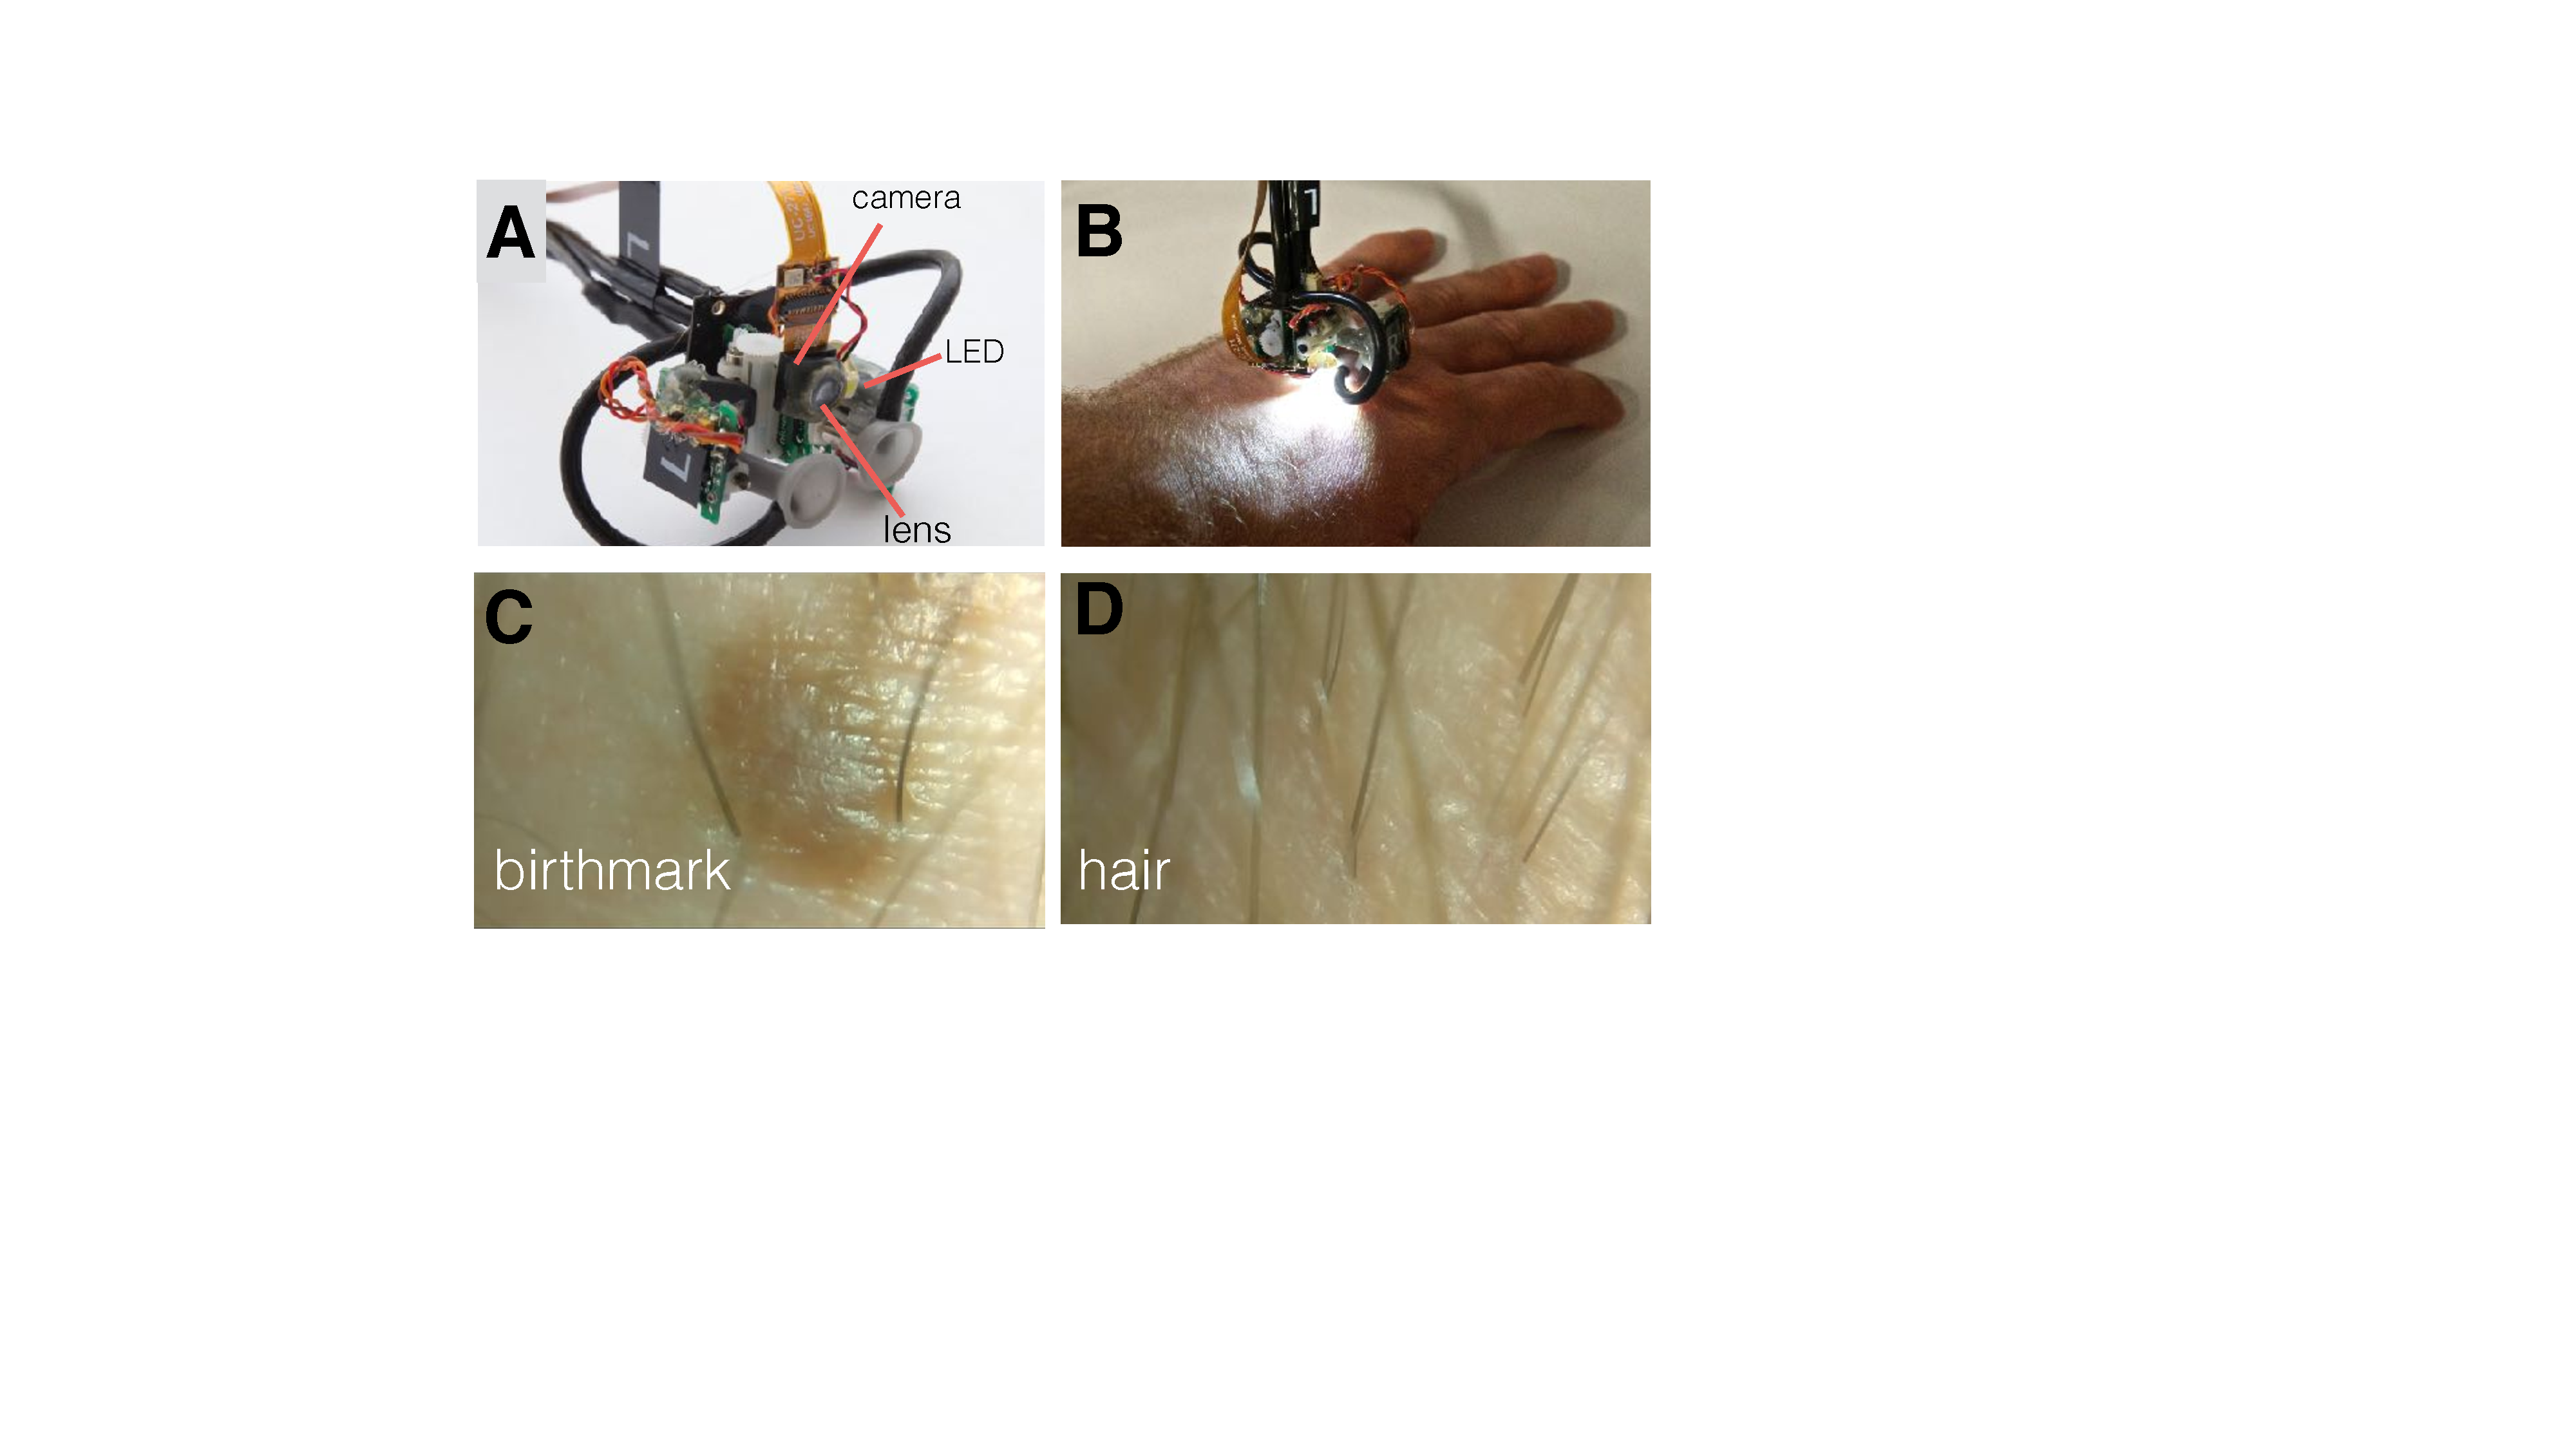
\includegraphics[width=0.9\columnwidth]{pictures/applications/visual_inspection.pdf}
\caption{Visual imaging of the skin. a) Bottom view of the robot showing the camera
sensing module. b) Epidermal robot using the camera module with a white LED for illumination. c) Camera snapshot showing a birthmark and d) Snapshot showing hair. }
\label{fig:visual_sensing}
\end{figure}

\begin{figure}[!t]
\centering
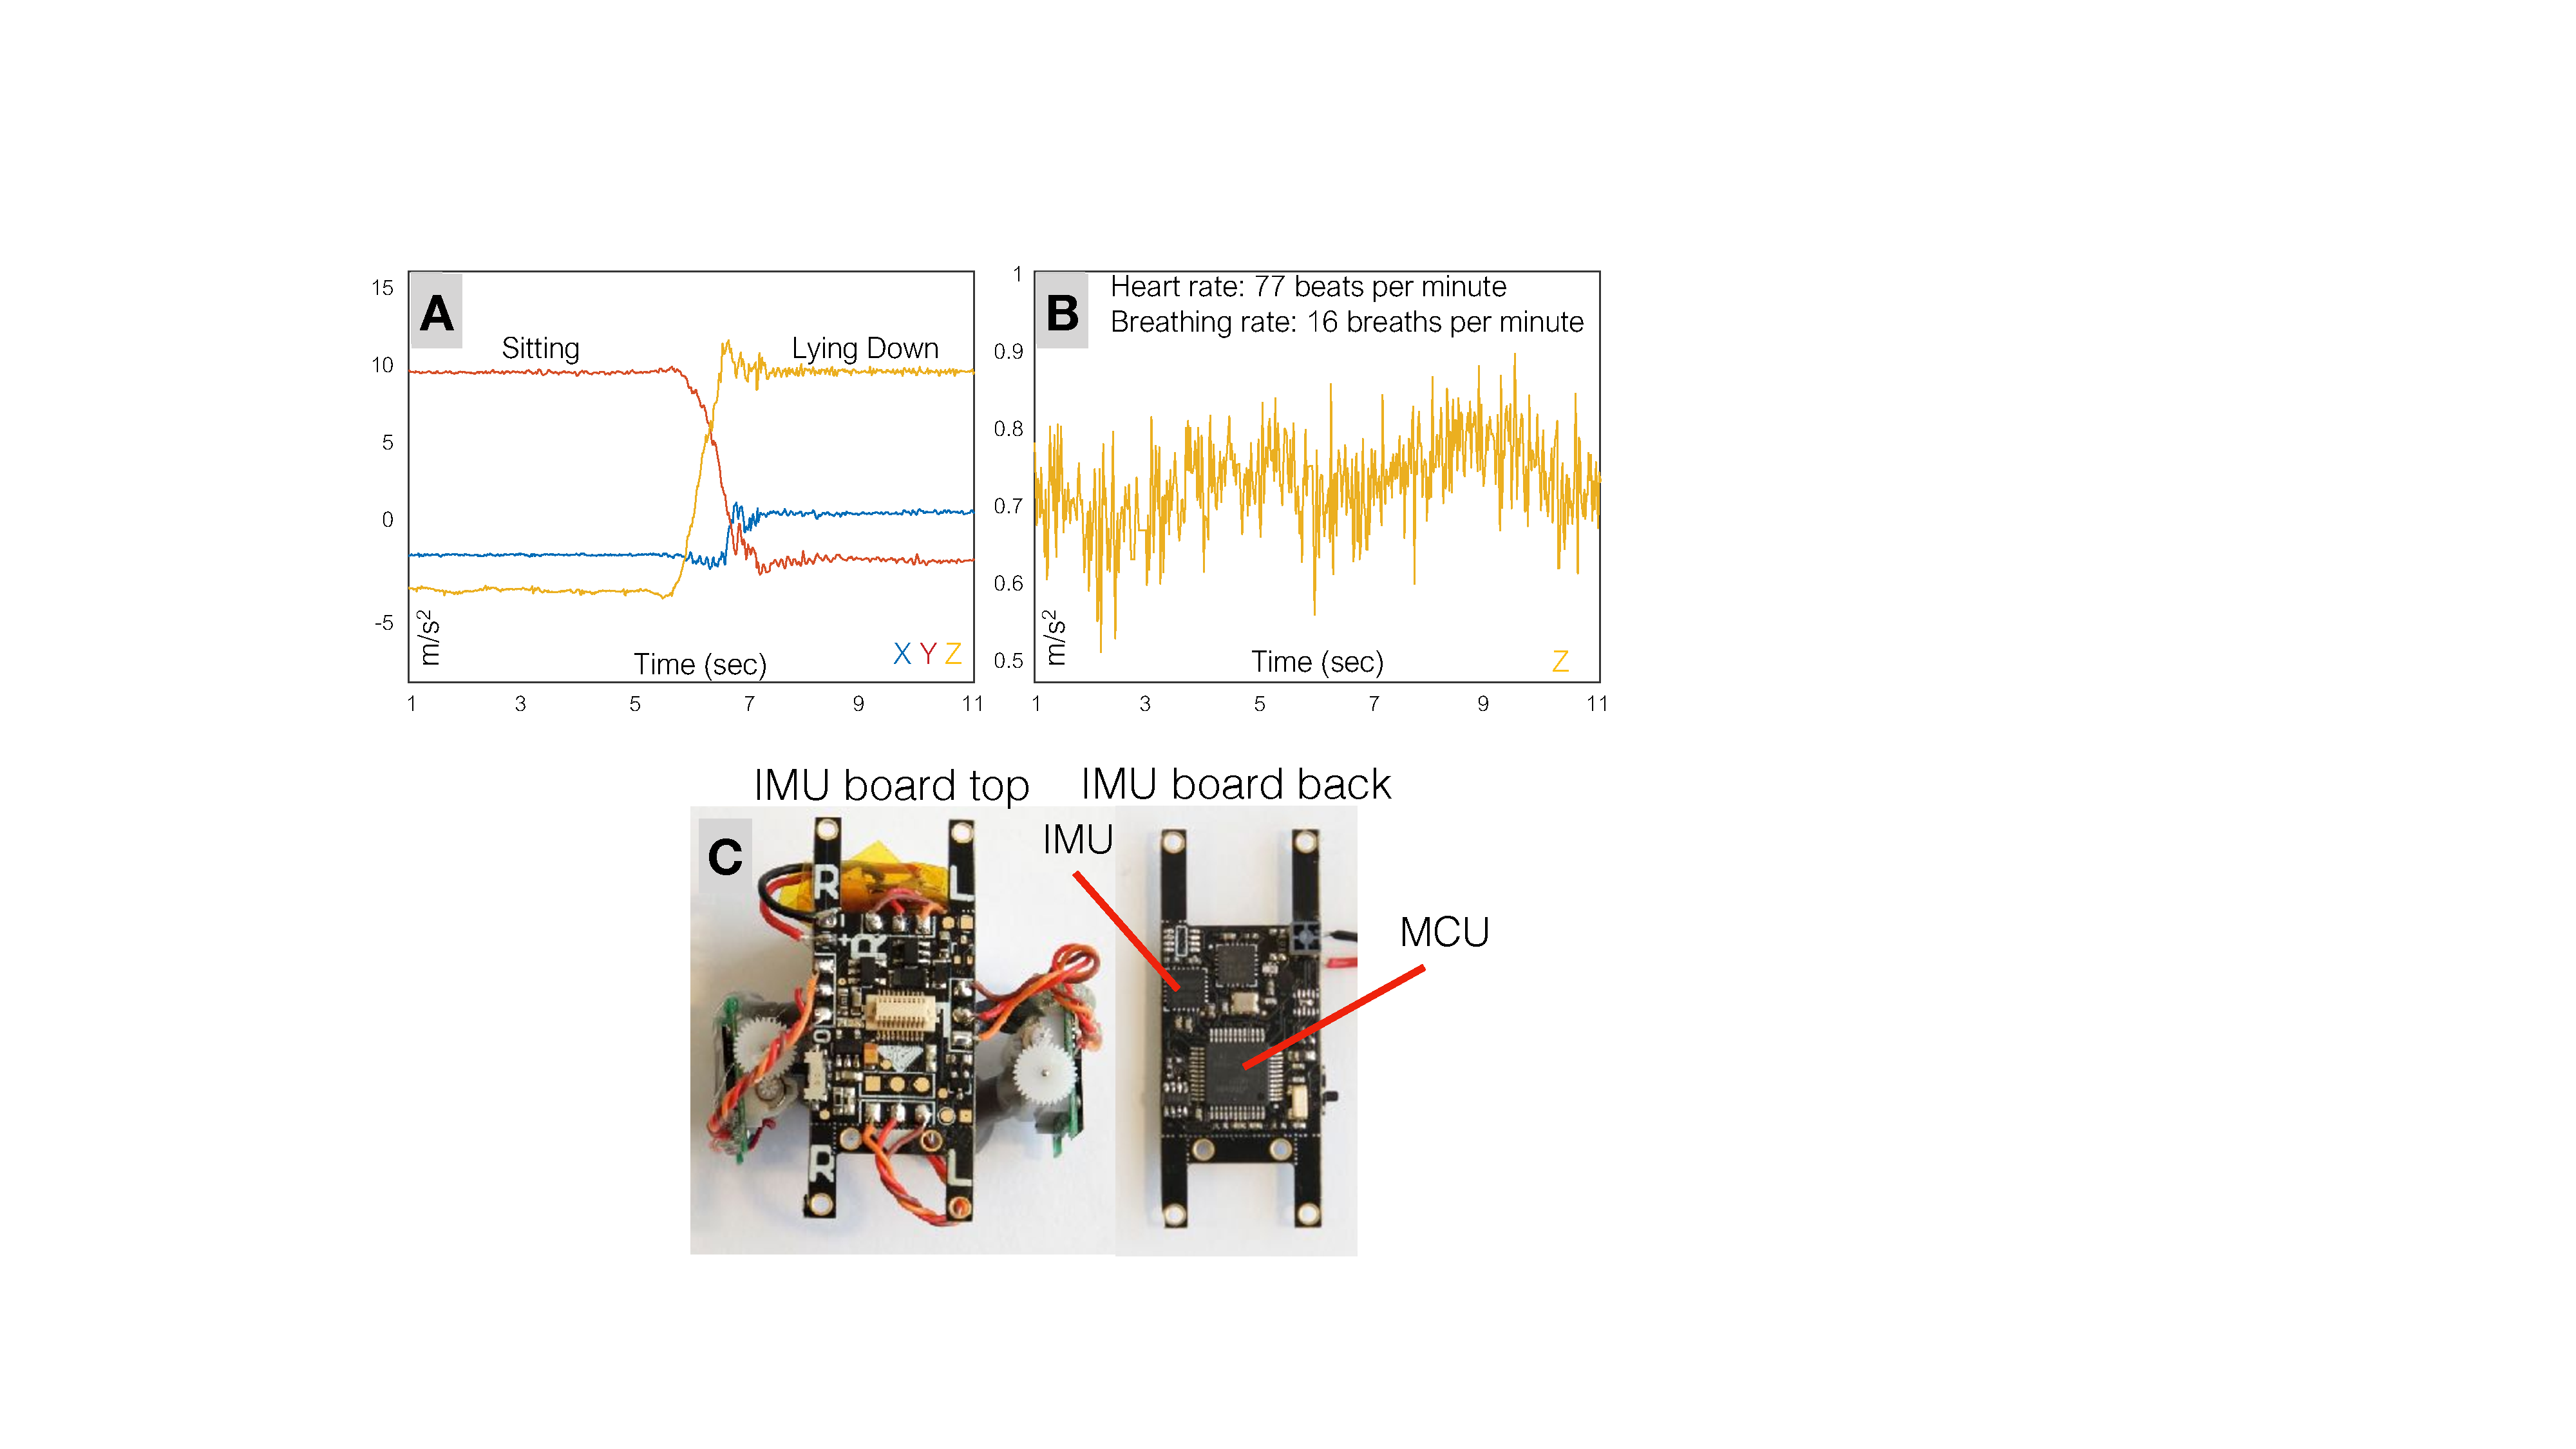
\includegraphics[width=0.9\columnwidth]{pictures/applications/IMU_sensing.pdf}
\caption{Inertial sensing with Epidermal robot: A) changes in accelerometer data during sitting and lying down position captured on the chest, and B), cardiorespiratory
motions captured on the chest. C), IMU board mounted on the robot. Backside of the IMU board contains a microcontroller (MCU) and a radio. IMU board also provides a connector to attach different modules such as an EKG module. }~\label{fig:imu_sensing}
\end{figure}

\subsection{Inertial Measurement Units}
Inertial measurement unit (IMU) is composed of accelerometer, gyroscope, and sometimes a magnetometer. The IMU is used for robot's navigation but can be used for applications such as motion capture, activity tracking and physiological sensing. As IMU tracks motions in relation to itself, it's position on the body is very important. For Epidermal robots and Rovables we used a 6-axis accelerometer and gyroscope (MPU6050, Invensense), sampled at 100 Hz.

Motion capture is used to record the movement of people or objects. Motion capture has many applications, such as medicine, sports, and gaming. Depending on its body location, IMUs have been used to track different activities (e.g., typing, steps, cycling) and body posture~\cite{attal2015physical}.  Most of the current systems use optical tracking, which has limited use, as it requires setting up cameras around the object. Although inertial motion capture systems use on-body sensors, they need a long process of placement and calibration of IMUs on each joint of the body (as many as 17 sensors). A shown in Figure~\ref{fig:skeleton}, Rovables can become a motion capture system, by using their IMUs. The process can be automated, as Rovables can travel to each joint and calibrate themselves. 

We developed a kinematic chain model of the human body using openFrameworks library~\cite{ofxSkeleton}. The data from IMUs were fed into inverse kinematics equations to track the positions of the joints.

The motion capture can be done with Epidermal robots and  Rovables as long as the clothing is not too loose. Attachment to the skin provides an ability to do physiological sensing of heart rate and breathing. 
Figure~\ref{fig:imu_sensing} shows accelerometer data captured while the Epidermal robot was on the chest of a person to capture different body postures and subtle cardiorespiratory vibrations from which heart and breathing rates are extracted~\cite{hernandez2015biophone}
 

 
 \begin{figure}[h]
\centering
  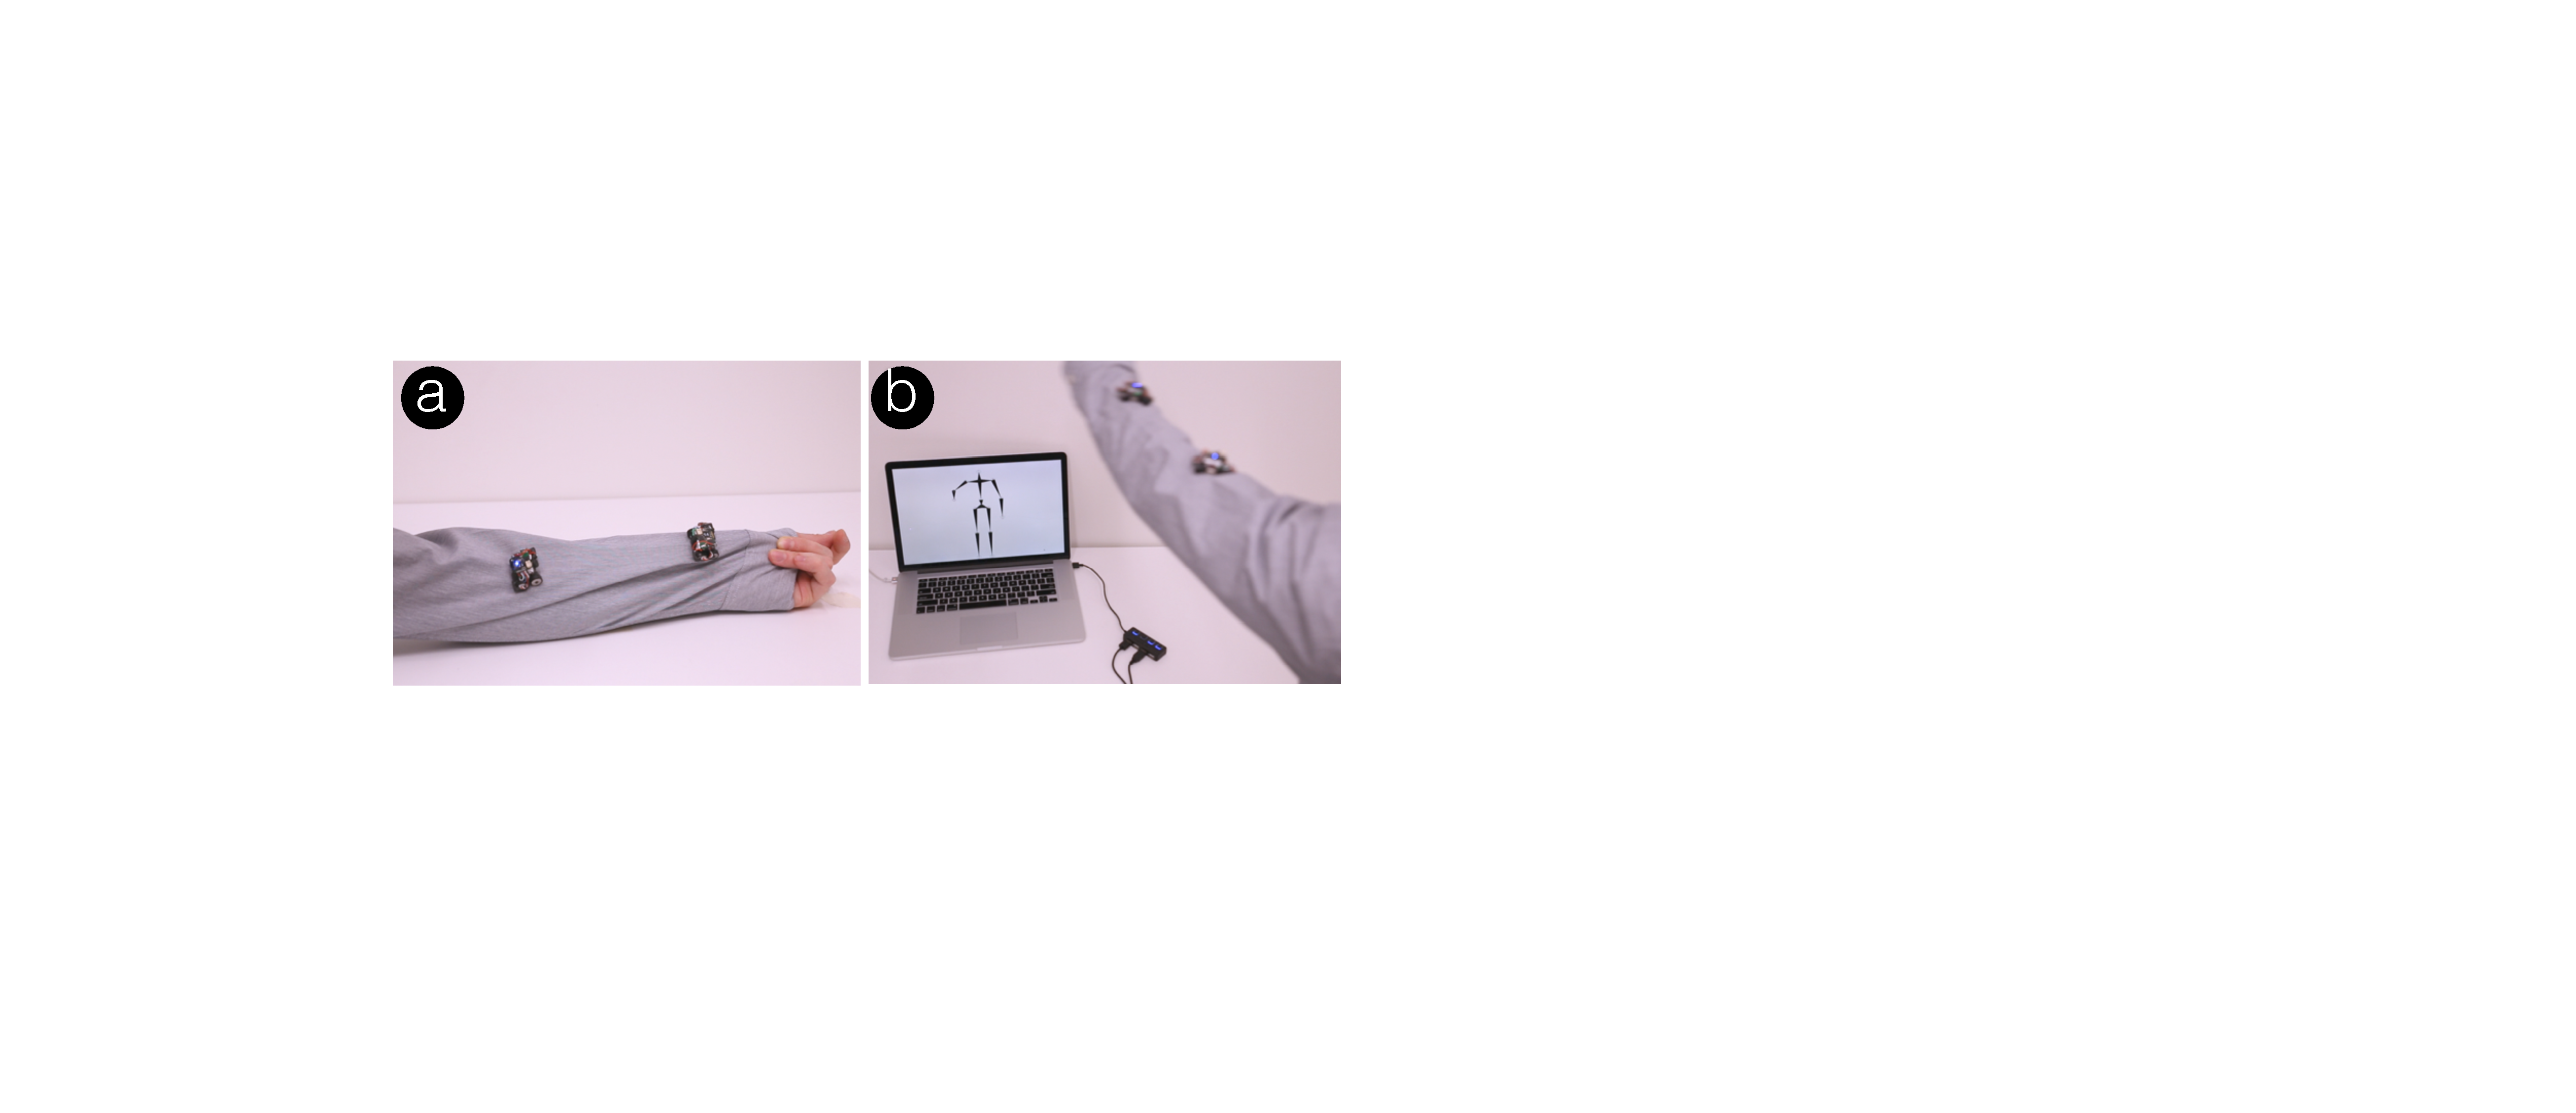
\includegraphics[width=1\columnwidth]{pictures/chapter4/skeleton.pdf}
  \caption{Using Rovables for motion capture. a) Rovables move to the right position on the arm. b) The kinematics of the arm is reconstructed on the screen. With more Rovables whole body skeleton can be reconstructed.}~\label{fig:skeleton}
\end{figure}


%%%%-----HCI-------
\section{Human-computer interactions}
Besides physiological sensing, wearable devices are often used for human-computer interactions, such as providing visual or tactile feedback. DWT can expand on such applications with its locomotion abilities. 

\subsection{Wearable displays}
We designed a display shield that connects to the expansion port on Rovables, as seen in Figure~\ref{fig:displays}. The shield adds a capacitive touch display with 63 RGB LEDs (Neopixel Mini). Also, it has an ATSAMD21G (Atmel) microcontroller, which allows playing and storing animations. On each side, the shield has IR LEDs and IR proximity sensors, so it can precisely connect with another LED shield or follow an IR beacon. To make it easier to link and align with another shield, each side has two magnets. The display allows us to develop and test scenarios and algorithms where Rovables cooperate to make a larger display. 

We developed a scenario where displays can become various output accessories. 
As an example, we developed an application scenario where one display-enabled robot is on a wrist and displays analog watch. When the user goes into a social situation, the robot moves to the chest and links up with another robot to form a name tag, as a larger display. When the user goes for a bicycle ride, the displays move to the back to form as safety turn lights.

\begin{figure}[h]
\centering
  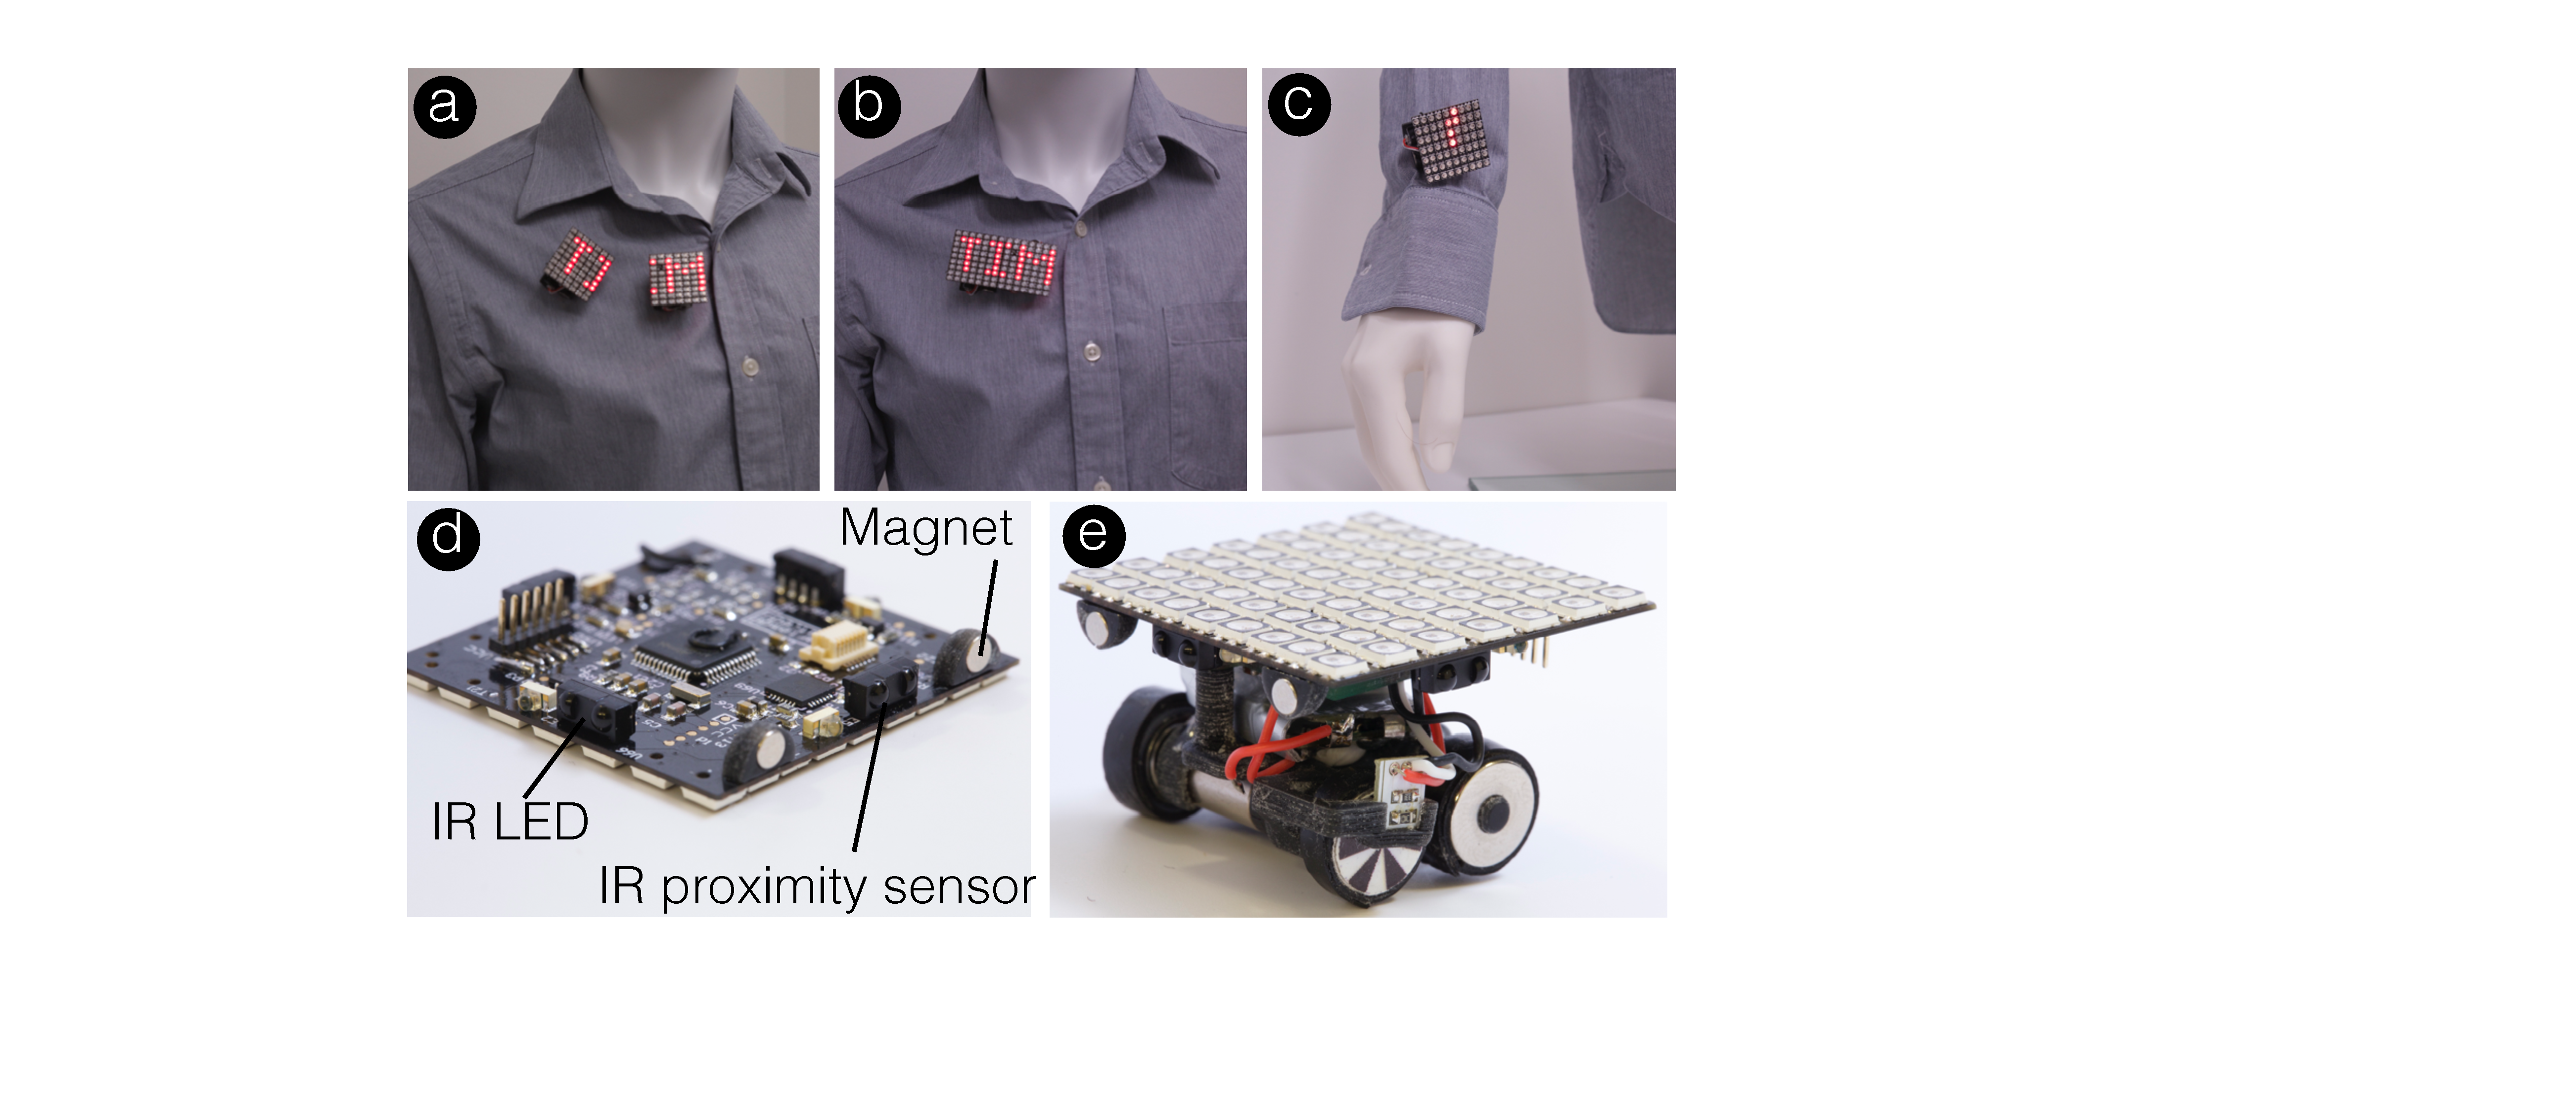
\includegraphics[width=1\columnwidth]{pictures/chapter4/displays_medium.pdf}
  \caption{Wearable displays application. a) and b)~The displays link together with magnets to form a larger name tag. c) The display can travel to the wrist to form a watch. d) The backside of the display shield exposes the IR beacon system and magnets for alignment with other displays. e) The Rovable with the attached display shield }~\label{fig:displays}
\end{figure}


\begin{figure}[!t]
\centering
  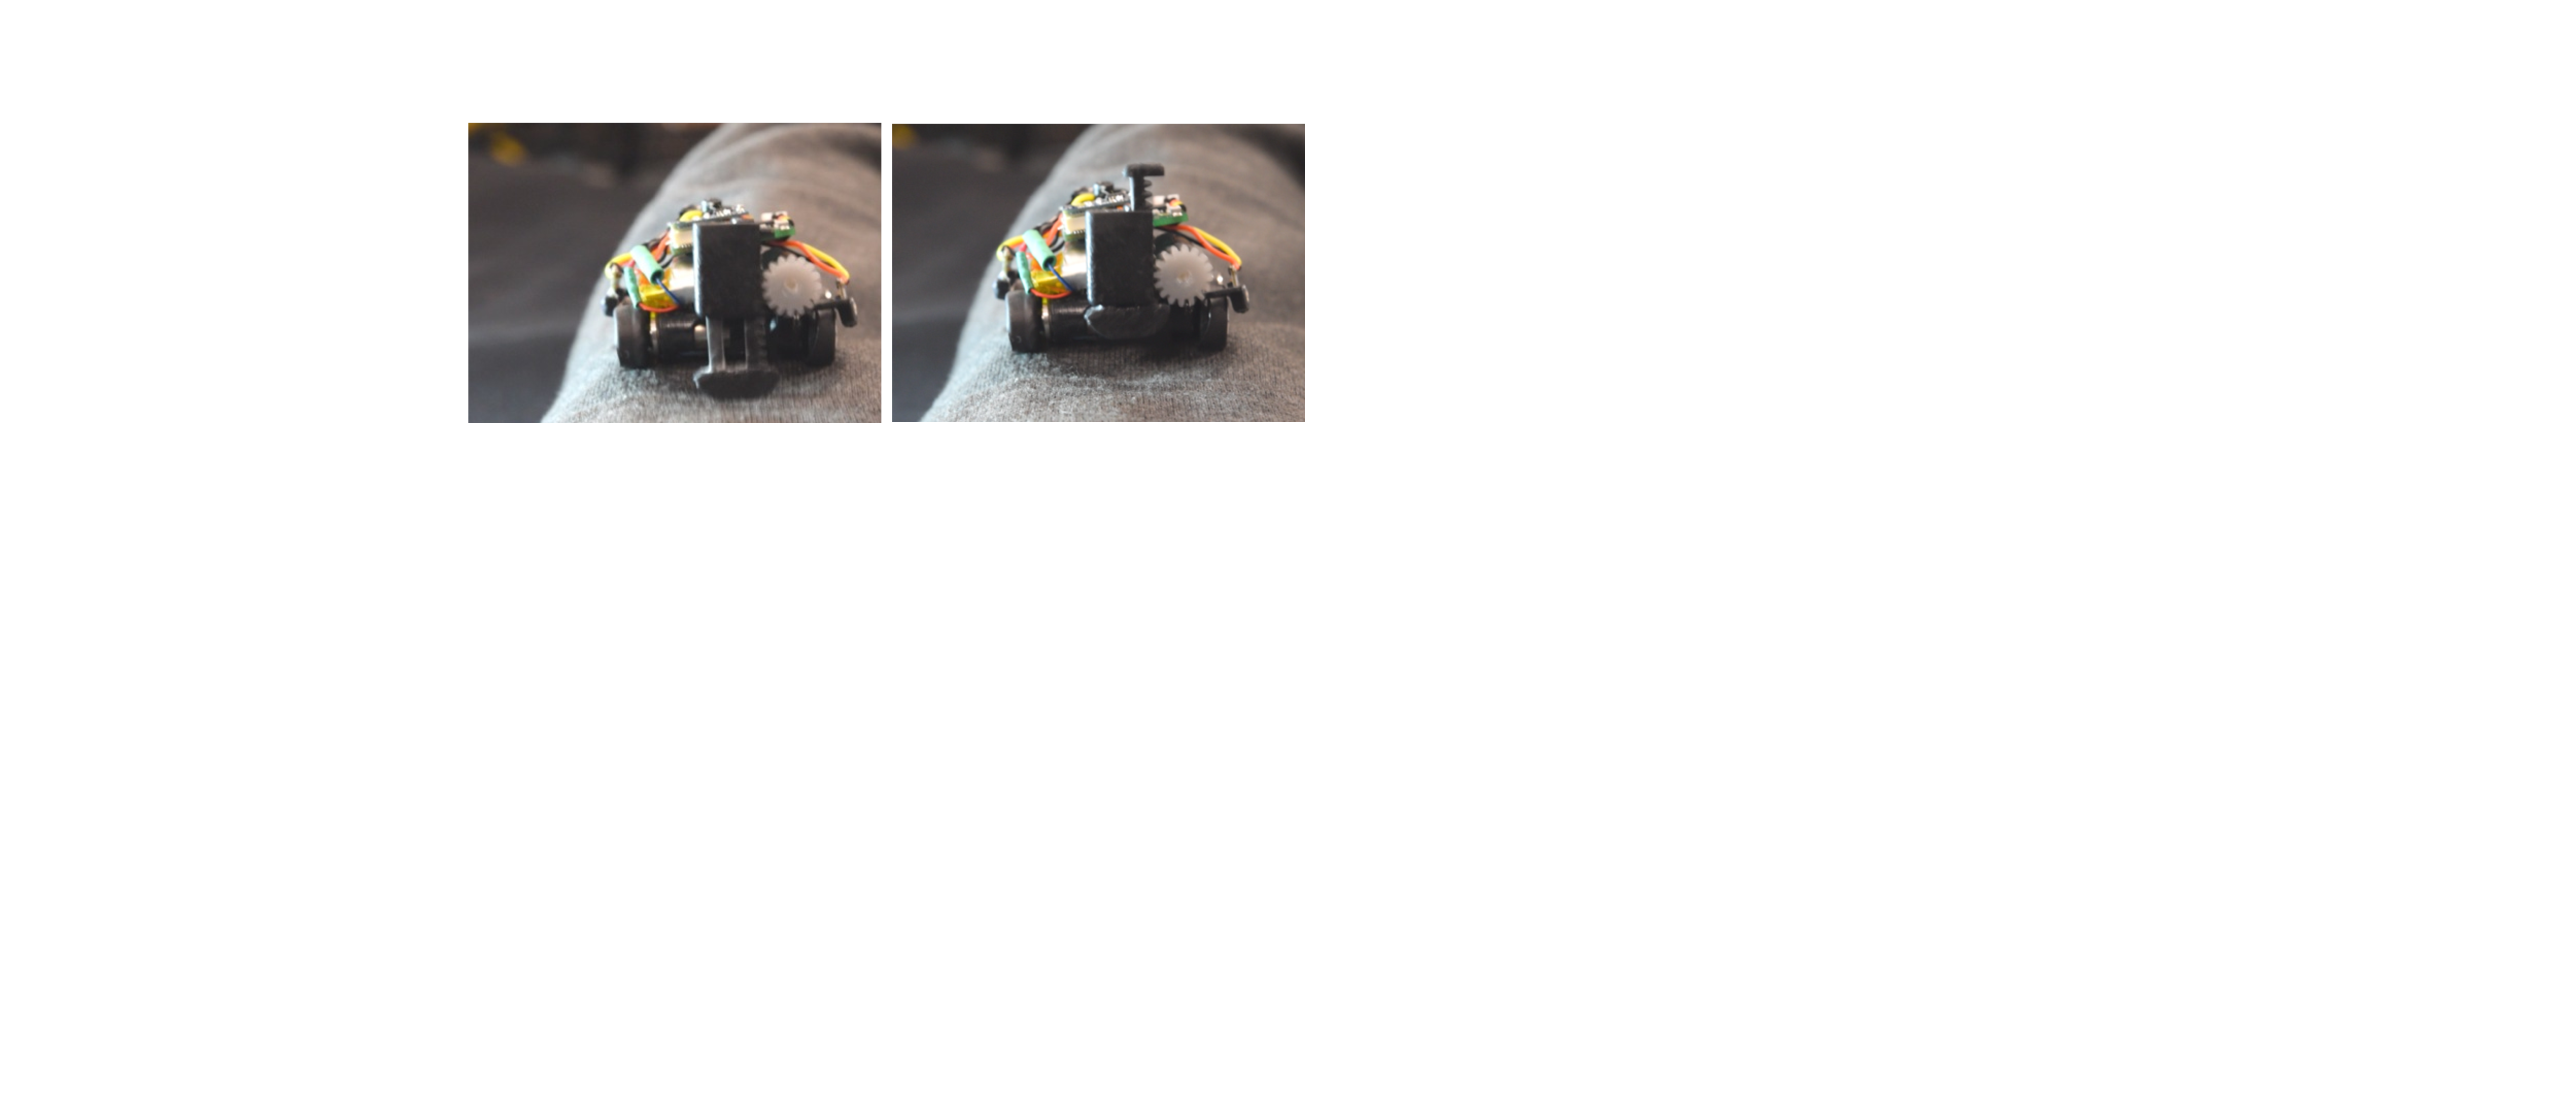
\includegraphics[width=1\columnwidth]{pictures/chapter4/linear_actuator.pdf}
  \caption{Tactile feedback application. We designed a linear actuator that can poke the skin. This tactor can go up and down to create tactile feedback.}~\label{fig:actuator}
\end{figure}

\subsection{Tactile Feedback}
Rovables can provide tactile feedback anywhere on the body. This is not possible with current wearable devices. To explore this idea, we designed a tactor that pokes the skin. The tactor is mounted on top of the Rovable, as shown in Figure~\ref{fig:actuator}. The tactor is driven by 136:1 small gear motor. A 3D-printed rack and pinion mechanism were used to convert the motor's circular motion into linear motion. 

The pushing force from the linear actuator is around 1N. But since the robot vibrates with the linear actuator, the actual force applied to the human body is less than 1N. To make a more effective tactor in the future, some stabilization mechanism for the robot will be required. 


\section{Design and art}
Because DWT is applied ultimately to the body, many design and art applications can arise. 

\subsection{Moving Fabric}
By attaching the robots to clothing, they can serve beyond individual roaming elements and expand to alter the shape of garment through movement. With the addition of a small Velcro hook on the robot casing, the robot attaches itself to the ends of a shawl which shape-changes into a scarf according to context, such as temperature change.  

\begin{figure}[!t]
\centering
  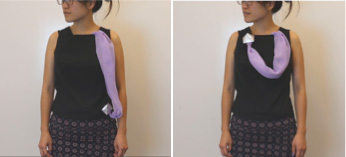
\includegraphics[width=1\columnwidth]{pictures/chapter4/scarf.jpg}
  \caption{Shape changing fabric. Robot self-attaches to fabric ends shifts to become a scarf according to temperature change.}~\label{fig:scarf}
\end{figure}

\subsection{Interactive Moving Jewelry}
Core interactions: ~\textit{Hiding interfaces, timed interfaces.}
With an aesthetic cover, the robot is transformed from a machine to a piece of jewelry, opening the space for decorative and functionally synthesized applications on the body. We present the example where the Rovable doubles as a brooch and microphone/speaker. It usually serves as a decorative brooch, yet when the wearer receives a phone call,  it shifts close to the neck to serve as a microphone/speaker in the case when the wearer's hands are full. 

\begin{figure}[h]
\centering
  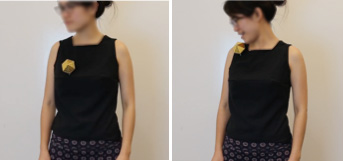
\includegraphics[width=1\columnwidth]{pictures/chapter4/speaker.jpg}
  \caption{Interactive moving jewelry. Robotic brooch moves to become a shoulder microphone speaker when wearer recieves phone call. }~\label{fig:speaker}
\end{figure}

\subsection{3D printing on the body}    
The robots could be used to 3D print on the body. This allows the clothing to be printed directly on the body. To test this concept, we created a proof of concept prototype that is based on FDM (fused deposition modeling) 3D printing. A prototype is shown in Figure~\ref{}. This technology deposits layers of hot thermoplastic filament.  We equipped the epidermal robot with an extruder nozzle and a mechanism to push the filament. The extruder was taken from a 3D doodler pen. 
For the filament, we used a low-temperature hot melt adhesive or hot glue. We selected this material as it was safe for skin use as it melted at low temperature (X C) and was safe for skin contact. 

\section{Summary}



